%%%%%%%%%%%%%%%%%%%%%%%%%%%%%%%%%%%%%%%%%
% The Legrand Orange Book
% LaTeX Template
% Version 2.0 (9/2/15)
% This template has been downloaded from:
% http://www.LaTeXTemplates.com
% Mathias Legrand (legrand.mathias@gmail.com) with modifications by:
% Vel (vel@latextemplates.com)
%
% License:
% CC BY-NC-SA 3.0 (http://creativecommons.org/licenses/by-nc-sa/3.0/)
%
% Important note:
% Chapter heading images should have a 2:1 width:height ratio,
% e.g. 920px width and 460px height.
%%%%%%%%%%%%%%%%%%%%%%%%%%%%%%%%%%%%%%%%%
%  Adaptado por Prof. Ausberto Castro Vera,
%  2013-2018
%----------------------------------------------------------------------------------------
%	PACKAGES AND OTHER DOCUMENT CONFIGURATIONS
%----------------------------------------------------------------------------------------

\documentclass[11pt,fleqn]{book} % Default font size and left-justified equations

%----------------------------------------------------------------------------------------

%%%%%%%%%%%%%%%%%%%%%%%%%%%%%%%%%%%%%%%%%
% The Legrand Orange Book
% Structural Definitions File
% Version 2.0 (9/2/15) 
%
% Original author:
% Mathias Legrand (legrand.mathias@gmail.com) with modifications by:
% Vel (vel@latextemplates.com)
%
% This file has been downloaded from:
% http://www.LaTeXTemplates.com
%
% License: 
% CC BY-NC-SA 3.0 (http://creativecommons.org/licenses/by-nc-sa/3.0/)
%
%%%%%%%%%%%%%%%%%%%%%%%%%%%%%%%%%%%%%%%%%%

%----------------------------------------------------------------------------------------
%	VARIOUS REQUIRED PACKAGES AND CONFIGURATIONS
%----------------------------------------------------------------------------------------

\usepackage[top=3cm,bottom=3cm,left=3cm,right=3cm,headsep=10pt,a4paper]{geometry} % Page margins

\usepackage{graphicx} % Required for including pictures
\graphicspath{{Pictures/}} % Specifies the directory where pictures are stored

\usepackage{lipsum} % Inserts dummy text
\usepackage{here}   %
\usepackage{tikz} % Required for drawing custom shapes

\usepackage[brazil]{babel} % Brazilian Portuguese language/hyphenation

\usepackage{enumitem} % Customize lists
\setlist{nolistsep} % Reduce spacing between bullet points and numbered lists

\usepackage{booktabs} % Required for nicer horizontal rules in tables

\usepackage{xcolor} % Required for specifying colors by name
\definecolor{ocre}{RGB}{243,102,25} % Define the orange color used for highlighting throughout the book

%----------------------------------------------------------------------------------------
%	FONTS
%----------------------------------------------------------------------------------------

\usepackage{avant} % Use the Avantgarde font for headings
%\usepackage{times} % Use the Times font for headings
\usepackage{mathptmx} % Use the Adobe Times Roman as the default text font together with math symbols from the Sym­bol, Chancery and Com­puter Modern fonts

\usepackage{microtype} % Slightly tweak font spacing for aesthetics
\usepackage[utf8]{inputenc} % Required for including letters with accents
\usepackage[T1]{fontenc} % Use 8-bit encoding that has 256 glyphs

%----------------------------------------------------------------------------------------
%	BIBLIOGRAPHY AND INDEX
%----------------------------------------------------------------------------------------
\usepackage{hyperref}

%\usepackage[style=alphabetic, citestyle=numeric, sorting=nyt, sortcites=true,
%            autopunct=true, babel=hyphen, hyperref=true, abbreviate=false,
%            backref=true, backend=biber]{biblatex}
%\addbibresource{racketbib.bib} % BibTeX bibliography file
%\defbibheading{bibempty}{}

\usepackage{calc} % For simpler calculation - used for spacing the index letter headings correctly
\usepackage{makeidx} % Required to make an index
\makeindex % Tells LaTeX to create the files required for indexing

%----------------------------------------------------------------------------------------
%	MAIN TABLE OF CONTENTS
%----------------------------------------------------------------------------------------

\usepackage{titletoc} % Required for manipulating the table of contents

\contentsmargin{0cm} % Removes the default margin

% Part text styling
\titlecontents{part}[0cm]
{\addvspace{20pt}\centering\large\bfseries}
{}
{}
{}

% Chapter text styling
\titlecontents{chapter}[1.25cm] % Indentation
{\addvspace{12pt}\large\sffamily\bfseries} % Spacing and font options for chapters
{\color{ocre!60}\contentslabel[\Large\thecontentslabel]{1.25cm}\color{ocre}} % Chapter number
{\color{ocre}}
{\color{ocre!60}\normalsize\;\titlerule*[.5pc]{.}\;\thecontentspage} % Page number

% Section text styling
\titlecontents{section}[1.25cm] % Indentation
{\addvspace{3pt}\sffamily\bfseries} % Spacing and font options for sections
{\contentslabel[\thecontentslabel]{1.25cm}} % Section number
{}
{\hfill\color{black}\thecontentspage} % Page number
[]

% Subsection text styling
\titlecontents{subsection}[1.25cm] % Indentation
{\addvspace{1pt}\sffamily\small} % Spacing and font options for subsections
{\contentslabel[\thecontentslabel]{1.25cm}} % Subsection number
{}
{\ \titlerule*[.5pc]{.}\;\thecontentspage} % Page number
[]

% List of figures
\titlecontents{figure}[0em]
{\addvspace{-5pt}\sffamily}
{\thecontentslabel\hspace*{1em}}
{}
{\ \titlerule*[.5pc]{.}\;\thecontentspage}
[]

% List of tables
\titlecontents{table}[0em]
{\addvspace{-5pt}\sffamily}
{\thecontentslabel\hspace*{1em}}
{}
{\ \titlerule*[.5pc]{.}\;\thecontentspage}
[]

%----------------------------------------------------------------------------------------
%	MINI TABLE OF CONTENTS IN PART HEADS
%----------------------------------------------------------------------------------------

% Chapter text styling
\titlecontents{lchapter}[0em] % Indenting
{\addvspace{15pt}\large\sffamily\bfseries} % Spacing and font options for chapters
{\color{ocre}\contentslabel[\Large\thecontentslabel]{1.25cm}\color{ocre}} % Chapter number
{}
{\color{ocre}\normalsize\sffamily\bfseries\;\titlerule*[.5pc]{.}\;\thecontentspage} % Page number

% Section text styling
\titlecontents{lsection}[0em] % Indenting
{\sffamily\small} % Spacing and font options for sections
{\contentslabel[\thecontentslabel]{1.25cm}} % Section number
{}
{}

% Subsection text styling
\titlecontents{lsubsection}[.5em] % Indentation
{\normalfont\footnotesize\sffamily} % Font settings
{}
{}
{}

%----------------------------------------------------------------------------------------
%	PAGE HEADERS
%----------------------------------------------------------------------------------------

\usepackage{fancyhdr} % Required for header and footer configuration

\pagestyle{fancy}
\renewcommand{\chaptermark}[1]{\markboth{\sffamily\normalsize\bfseries\chaptername\ \thechapter.\ #1}{}} % Chapter text font settings
\renewcommand{\sectionmark}[1]{\markright{\sffamily\normalsize\thesection\hspace{5pt}#1}{}} % Section text font settings
\fancyhf{} \fancyhead[LE,RO]{\sffamily\normalsize\thepage} % Font setting for the page number in the header
\fancyhead[LO]{\rightmark} % Print the nearest section name on the left side of odd pages
\fancyhead[RE]{\leftmark} % Print the current chapter name on the right side of even pages
\renewcommand{\headrulewidth}{0.5pt} % Width of the rule under the header
\addtolength{\headheight}{2.5pt} % Increase the spacing around the header slightly
\renewcommand{\footrulewidth}{0pt} % Removes the rule in the footer
\fancypagestyle{plain}{\fancyhead{}\renewcommand{\headrulewidth}{0pt}} % Style for when a plain pagestyle is specified

% Removes the header from odd empty pages at the end of chapters
\makeatletter
\renewcommand{\cleardoublepage}{
\clearpage\ifodd\c@page\else
\hbox{}
\vspace*{\fill}
\thispagestyle{empty}
\newpage
\fi}

%----------------------------------------------------------------------------------------
%	THEOREM STYLES
%----------------------------------------------------------------------------------------

\usepackage{amsmath,amsfonts,amssymb,amsthm} % For math equations, theorems, symbols, etc

\newcommand{\intoo}[2]{\mathopen{]}#1\,;#2\mathclose{[}}
\newcommand{\ud}{\mathop{\mathrm{{}d}}\mathopen{}}
\newcommand{\intff}[2]{\mathopen{[}#1\,;#2\mathclose{]}}
\newtheorem{notation}{Notation}[chapter]

% Boxed/framed environments
\newtheoremstyle{ocrenumbox}% % Theorem style name
{0pt}% Space above
{0pt}% Space below
{\normalfont}% % Body font
{}% Indent amount
{\small\bf\sffamily\color{ocre}}% % Theorem head font
{\;}% Punctuation after theorem head
{0.25em}% Space after theorem head
{\small\sffamily\color{ocre}\thmname{#1}\nobreakspace\thmnumber{\@ifnotempty{#1}{}\@upn{#2}}% Theorem text (e.g. Theorem 2.1)
\thmnote{\nobreakspace\the\thm@notefont\sffamily\bfseries\color{black}---\nobreakspace#3.}} % Optional theorem note
\renewcommand{\qedsymbol}{$\blacksquare$}% Optional qed square

\newtheoremstyle{blacknumex}% Theorem style name
{5pt}% Space above
{5pt}% Space below
{\normalfont}% Body font
{} % Indent amount
{\small\bf\sffamily}% Theorem head font
{\;}% Punctuation after theorem head
{0.25em}% Space after theorem head
{\small\sffamily{\tiny\ensuremath{\blacksquare}}\nobreakspace\thmname{#1}\nobreakspace\thmnumber{\@ifnotempty{#1}{}\@upn{#2}}% Theorem text (e.g. Theorem 2.1)
\thmnote{\nobreakspace\the\thm@notefont\sffamily\bfseries---\nobreakspace#3.}}% Optional theorem note

\newtheoremstyle{blacknumbox} % Theorem style name
{0pt}% Space above
{0pt}% Space below
{\normalfont}% Body font
{}% Indent amount
{\small\bf\sffamily}% Theorem head font
{\;}% Punctuation after theorem head
{0.25em}% Space after theorem head
{\small\sffamily\thmname{#1}\nobreakspace\thmnumber{\@ifnotempty{#1}{}\@upn{#2}}% Theorem text (e.g. Theorem 2.1)
\thmnote{\nobreakspace\the\thm@notefont\sffamily\bfseries---\nobreakspace#3.}}% Optional theorem note

% Non-boxed/non-framed environments
\newtheoremstyle{ocrenum}% % Theorem style name
{5pt}% Space above
{5pt}% Space below
{\normalfont}% % Body font
{}% Indent amount
{\small\bf\sffamily\color{ocre}}% % Theorem head font
{\;}% Punctuation after theorem head
{0.25em}% Space after theorem head
{\small\sffamily\color{ocre}\thmname{#1}\nobreakspace\thmnumber{\@ifnotempty{#1}{}\@upn{#2}}% Theorem text (e.g. Theorem 2.1)
\thmnote{\nobreakspace\the\thm@notefont\sffamily\bfseries\color{black}---\nobreakspace#3.}} % Optional theorem note
\renewcommand{\qedsymbol}{$\blacksquare$}% Optional qed square
\makeatother

% Defines the theorem text style for each type of theorem to one of the three styles above
\newcounter{dummy}
\numberwithin{dummy}{section}
\theoremstyle{ocrenumbox}
\newtheorem{theoremeT}[dummy]{Theorem}
\newtheorem{problem}{Problem}[chapter]
\newtheorem{exerciseT}{Exercise}[chapter]
\theoremstyle{blacknumex}
\newtheorem{exampleT}{Example}[chapter]
\theoremstyle{blacknumbox}
\newtheorem{vocabulary}{Vocabulary}[chapter]
\newtheorem{definitionT}{Definition}[section]
\newtheorem{corollaryT}[dummy]{Corollary}
\theoremstyle{ocrenum}
\newtheorem{proposition}[dummy]{Proposition}

%----------------------------------------------------------------------------------------
%	DEFINITION OF COLORED BOXES
%----------------------------------------------------------------------------------------

\RequirePackage[framemethod=default]{mdframed} % Required for creating the theorem, definition, exercise and corollary boxes

% Theorem box
\newmdenv[skipabove=7pt,
skipbelow=7pt,
backgroundcolor=black!5,
linecolor=ocre,
innerleftmargin=5pt,
innerrightmargin=5pt,
innertopmargin=5pt,
leftmargin=0cm,
rightmargin=0cm,
innerbottommargin=5pt]{tBox}

% Exercise box	
\newmdenv[skipabove=7pt,
skipbelow=7pt,
rightline=false,
leftline=true,
topline=false,
bottomline=false,
backgroundcolor=ocre!10,
linecolor=ocre,
innerleftmargin=5pt,
innerrightmargin=5pt,
innertopmargin=5pt,
innerbottommargin=5pt,
leftmargin=0cm,
rightmargin=0cm,
linewidth=4pt]{eBox}	

% Definition box
\newmdenv[skipabove=7pt,
skipbelow=7pt,
rightline=false,
leftline=true,
topline=false,
bottomline=false,
linecolor=ocre,
innerleftmargin=5pt,
innerrightmargin=5pt,
innertopmargin=0pt,
leftmargin=0cm,
rightmargin=0cm,
linewidth=4pt,
innerbottommargin=0pt]{dBox}	

% Corollary box
\newmdenv[skipabove=7pt,
skipbelow=7pt,
rightline=false,
leftline=true,
topline=false,
bottomline=false,
linecolor=gray,
backgroundcolor=black!5,
innerleftmargin=5pt,
innerrightmargin=5pt,
innertopmargin=5pt,
leftmargin=0cm,
rightmargin=0cm,
linewidth=4pt,
innerbottommargin=5pt]{cBox}

% Creates an environment for each type of theorem and assigns it a theorem text style from the "Theorem Styles" section above and a colored box from above
\newenvironment{theorem}{\begin{tBox}\begin{theoremeT}}{\end{theoremeT}\end{tBox}}
\newenvironment{exercise}{\begin{eBox}\begin{exerciseT}}{\hfill{\color{ocre}\tiny\ensuremath{\blacksquare}}\end{exerciseT}\end{eBox}}				
\newenvironment{definition}{\begin{dBox}\begin{definitionT}}{\end{definitionT}\end{dBox}}	
\newenvironment{example}{\begin{exampleT}}{\hfill{\tiny\ensuremath{\blacksquare}}\end{exampleT}}		
\newenvironment{corollary}{\begin{cBox}\begin{corollaryT}}{\end{corollaryT}\end{cBox}}	

%----------------------------------------------------------------------------------------
%	REMARK ENVIRONMENT
%----------------------------------------------------------------------------------------

\newenvironment{remark}{\par\vspace{10pt}\small % Vertical white space above the remark and smaller font size
\begin{list}{}{
\leftmargin=35pt % Indentation on the left
\rightmargin=25pt}\item\ignorespaces % Indentation on the right
\makebox[-2.5pt]{\begin{tikzpicture}[overlay]
\node[draw=ocre!60,line width=1pt,circle,fill=ocre!25,font=\sffamily\bfseries,inner sep=2pt,outer sep=0pt] at (-15pt,0pt){\textcolor{ocre}{R}};\end{tikzpicture}} % Orange R in a circle
\advance\baselineskip -1pt}{\end{list}\vskip5pt} % Tighter line spacing and white space after remark

%----------------------------------------------------------------------------------------
%	SECTION NUMBERING IN THE MARGIN
%----------------------------------------------------------------------------------------

\makeatletter
\renewcommand{\@seccntformat}[1]{\llap{\textcolor{ocre}{\csname the#1\endcsname}\hspace{1em}}}
\renewcommand{\section}{\@startsection{section}{1}{\z@}
{-4ex \@plus -1ex \@minus -.4ex}
{1ex \@plus.2ex }
{\normalfont\large\sffamily\bfseries}}
\renewcommand{\subsection}{\@startsection {subsection}{2}{\z@}
{-3ex \@plus -0.1ex \@minus -.4ex}
{0.5ex \@plus.2ex }
{\normalfont\sffamily\bfseries}}
\renewcommand{\subsubsection}{\@startsection {subsubsection}{3}{\z@}
{-2ex \@plus -0.1ex \@minus -.2ex}
{.2ex \@plus.2ex }
{\normalfont\small\sffamily\bfseries}}
\renewcommand\paragraph{\@startsection{paragraph}{4}{\z@}
{-2ex \@plus-.2ex \@minus .2ex}
{.1ex}
{\normalfont\small\sffamily\bfseries}}

%----------------------------------------------------------------------------------------
%	PART HEADINGS
%----------------------------------------------------------------------------------------

% numbered part in the table of contents
\newcommand{\@mypartnumtocformat}[2]{%
\setlength\fboxsep{0pt}%
\noindent\colorbox{ocre!20}{\strut\parbox[c][.7cm]{\ecart}{\color{ocre!70}\Large\sffamily\bfseries\centering#1}}\hskip\esp\colorbox{ocre!40}{\strut\parbox[c][.7cm]{\linewidth-\ecart-\esp}{\Large\sffamily\centering#2}}}%
%%%%%%%%%%%%%%%%%%%%%%%%%%%%%%%%%%
% unnumbered part in the table of contents
\newcommand{\@myparttocformat}[1]{%
\setlength\fboxsep{0pt}%
\noindent\colorbox{ocre!40}{\strut\parbox[c][.7cm]{\linewidth}{\Large\sffamily\centering#1}}}%
%%%%%%%%%%%%%%%%%%%%%%%%%%%%%%%%%%
\newlength\esp
\setlength\esp{4pt}
\newlength\ecart
\setlength\ecart{1.2cm-\esp}
\newcommand{\thepartimage}{}%
\newcommand{\partimage}[1]{\renewcommand{\thepartimage}{#1}}%
\def\@part[#1]#2{%
\ifnum \c@secnumdepth >-2\relax%
\refstepcounter{part}%
\addcontentsline{toc}{part}{\texorpdfstring{\protect\@mypartnumtocformat{\thepart}{#1}}{\partname~\thepart\ ---\ #1}}
\else%
\addcontentsline{toc}{part}{\texorpdfstring{\protect\@myparttocformat{#1}}{#1}}%
\fi%
\startcontents%
\markboth{}{}%
{\thispagestyle{empty}%
\begin{tikzpicture}[remember picture,overlay]%
\node at (current page.north west){\begin{tikzpicture}[remember picture,overlay]%	
\fill[ocre!20](0cm,0cm) rectangle (\paperwidth,-\paperheight);
\node[anchor=north] at (4cm,-3.25cm){\color{ocre!40}\fontsize{220}{100}\sffamily\bfseries\@Roman\c@part};
\node[anchor=south east] at (\paperwidth-1cm,-\paperheight+1cm){\parbox[t][][t]{8.5cm}{
\printcontents{l}{0}{\setcounter{tocdepth}{1}}%
}};
\node[anchor=north east] at (\paperwidth-1.5cm,-3.25cm){\parbox[t][][t]{15cm}{\strut\raggedleft\color{white}\fontsize{30}{30}\sffamily\bfseries#2}};
\end{tikzpicture}};
\end{tikzpicture}}%
\@endpart}
\def\@spart#1{%
\startcontents%
\phantomsection
{\thispagestyle{empty}%
\begin{tikzpicture}[remember picture,overlay]%
\node at (current page.north west){\begin{tikzpicture}[remember picture,overlay]%	
\fill[ocre!20](0cm,0cm) rectangle (\paperwidth,-\paperheight);
\node[anchor=north east] at (\paperwidth-1.5cm,-3.25cm){\parbox[t][][t]{15cm}{\strut\raggedleft\color{white}\fontsize{30}{30}\sffamily\bfseries#1}};
\end{tikzpicture}};
\end{tikzpicture}}
\addcontentsline{toc}{part}{\texorpdfstring{%
\setlength\fboxsep{0pt}%
\noindent\protect\colorbox{ocre!40}{\strut\protect\parbox[c][.7cm]{\linewidth}{\Large\sffamily\protect\centering #1\quad\mbox{}}}}{#1}}%
\@endpart}
\def\@endpart{\vfil\newpage
\if@twoside
\if@openright
\null
\thispagestyle{empty}%
\newpage
\fi
\fi
\if@tempswa
\twocolumn
\fi}

%----------------------------------------------------------------------------------------
%	CHAPTER HEADINGS
%----------------------------------------------------------------------------------------

\newcommand{\thechapterimage}{}%
\newcommand{\chapterimage}[1]{\renewcommand{\thechapterimage}{#1}}%
\def\@makechapterhead#1{%
{\parindent \z@ \raggedright \normalfont
\ifnum \c@secnumdepth >\m@ne
\if@mainmatter
\begin{tikzpicture}[remember picture,overlay]
\node at (current page.north west)
{\begin{tikzpicture}[remember picture,overlay]
\node[anchor=north west,inner sep=0pt] at (0,0) {\includegraphics[width=\paperwidth]{\thechapterimage}};
\draw[anchor=west] (\Gm@lmargin,-9cm) node [line width=2pt,rounded corners=15pt,draw=ocre,fill=white,fill opacity=0.5,inner sep=15pt]{\strut\makebox[22cm]{}};
\draw[anchor=west] (\Gm@lmargin+.3cm,-9cm) node {\huge\sffamily\bfseries\color{black}\thechapter. #1\strut};
\end{tikzpicture}};
\end{tikzpicture}
\else
\begin{tikzpicture}[remember picture,overlay]
\node at (current page.north west)
{\begin{tikzpicture}[remember picture,overlay]
\node[anchor=north west,inner sep=0pt] at (0,0) {\includegraphics[width=\paperwidth]{\thechapterimage}};
\draw[anchor=west] (\Gm@lmargin,-9cm) node [line width=2pt,rounded corners=15pt,draw=ocre,fill=white,fill opacity=0.5,inner sep=15pt]{\strut\makebox[22cm]{}};
\draw[anchor=west] (\Gm@lmargin+.3cm,-9cm) node {\huge\sffamily\bfseries\color{black}#1\strut};
\end{tikzpicture}};
\end{tikzpicture}
\fi\fi\par\vspace*{270\p@}}}

%-------------------------------------------

\def\@makeschapterhead#1{%
\begin{tikzpicture}[remember picture,overlay]
\node at (current page.north west)
{\begin{tikzpicture}[remember picture,overlay]
\node[anchor=north west,inner sep=0pt] at (0,0) {\includegraphics[width=\paperwidth]{\thechapterimage}};
\draw[anchor=west] (\Gm@lmargin,-9cm) node [line width=2pt,rounded corners=15pt,draw=ocre,fill=white,fill opacity=0.5,inner sep=15pt]{\strut\makebox[22cm]{}};
\draw[anchor=west] (\Gm@lmargin+.3cm,-9cm) node {\huge\sffamily\bfseries\color{black}#1\strut};
\end{tikzpicture}};
\end{tikzpicture}
\par\vspace*{270\p@}}
\makeatother

%----------------------------------------------------------------------------------------
%	HYPERLINKS IN THE DOCUMENTS
%----------------------------------------------------------------------------------------

\usepackage{hyperref}
\hypersetup{hidelinks,backref=true,pagebackref=true,hyperindex=true,colorlinks=false,breaklinks=true,urlcolor= ocre,bookmarks=true,bookmarksopen=false,pdftitle={Title},pdfauthor={Author}}
\usepackage{bookmark}
\bookmarksetup{
open,
numbered,
addtohook={%
\ifnum\bookmarkget{level}=0 % chapter
\bookmarksetup{bold}%
\fi
\ifnum\bookmarkget{level}=-1 % part
\bookmarksetup{color=ocre,bold}%
\fi
}
}
\usepackage{setspace}
\usepackage[many]{tcolorbox}
\tcbset{skin=enhanced}


\usepackage{listings}
         \lstset{ %
  	      language={Python}, %Pascal % lenguaje de programaci\'{o}n
  	      basicstyle=\bfseries\ttfamily,
  	      keywordstyle=\color{blue},
  	      commentstyle=\color{brown},	
  	      backgroundcolor=\color{green!10},
  	      showstringspaces=false
  	      }

\usepackage[brazilian,hyperpageref]{backref}
% Configurações do pacote backref
% Usado sem a opção hyperpageref de backref
\renewcommand{\backrefpagesname}{Citado nas páginas:}
% Texto padr\~{a}o antes do número das páginas
\renewcommand{\backref}{}
% Define os textos da citação
\renewcommand*{\backrefalt}[4]{
	\ifcase #1 %
		Nenhuma citação no texto.%
	\or
		Citado na página #2.%
	\else
		Citado #1 vezes nas páginas #2.%
	\fi}%
% ---


\sloppy


\hypersetup{
    bookmarks=true,         % show bookmarks bar?
    unicode=false,          % non-Latin characters in Acrobat’s bookmarks
    pdftoolbar=true,        % show Acrobat’s toolbar?
    pdfmenubar=true,        % show Acrobat’s menu?
    pdffitwindow=true,     % window fit to page when opened
    pdfstartview={FitH},    % fits the width of the page to the window
    pdftitle={Tutorial sobre a Linguagem Racket},    % title
  %  pdfauthor={Mariana A. Gualhano and Ausberto S. Castro Vera},     % author
    pdfsubject={Paradigmas de Linguagens de Programa\c{c}\~{a}o},   % subject of the document
    pdfcreator={ASCV, WinEdt},   % creator of the document
    pdfproducer={ASCV}, % producer of the document
    pdfkeywords={Programa\c{c}\~{a}o} {Funcional} {Paradigmas}, % list of keywords
    pdfnewwindow=true,      % links in new window
    colorlinks=true,       % false: boxed links; true: colored links
    linkcolor=ocre,          % color of internal links (change box color with linkbordercolor)
    citecolor=blue,        % color of links to bibliography
    filecolor=magenta,      % color of file links
    urlcolor=cyan           % color of external links
}	
 % Insert the commands.tex file which contains the majority of the structure behind the template

\begin{document}

%----------------------------------------------------------------------------------------
%	TITLE PAGE
%----------------------------------------------------------------------------------------

\begingroup
\thispagestyle{empty}
\begin{tikzpicture}[remember picture,overlay]
\coordinate [below=12cm] (midpoint) at (current page.north);
\node at (current page.north west)
{\begin{tikzpicture}[remember picture,overlay]
\node[anchor=north west,inner sep=0pt] at (0,0)
        {
\includegraphics[width=\paperwidth]{capa.png}}; %Capa Imagem A4 21x29.7
\draw[anchor=north] (midpoint) node [fill=ocre!30!white,fill opacity=0.6,text opacity=1,inner sep=1cm]{\Huge\centering\bfseries\sffamily\parbox[c][][t]
        {\paperwidth}
        {\centering Introdu\c{c}\~{a}o \`{a} Linguagem Python\\[5pt] % Titulo Livro
{\Large Paradigmas de Linguagens de Programa\c{c}\~{a}o}\\[20pt] % Subtitle
{\huge \color{blue} Mariana Cossetti Dalfior}\\ % Autor nome
{\huge  \color{blue}  Ausberto S. Castro Vera}\\
{\small \today}
}}; % Autor nome
\end{tikzpicture}};
\end{tikzpicture}
\vfill

\endgroup
 
%----------------------------------------------------------------------------------------
%	COPYRIGHT PAGE
%----------------------------------------------------------------------------------------


\newpage
% Prof. Dr. Ausberto S. Castro Vera
% UENF - CCT - LCMAT - Curso de Ci\^{e}ncia da Computa\c{c}\~{a}o
% Campos, RJ,  2023
% Disciplina: Paradigmas de Linguagens de Programa\c{c}\~{a}o
% Aluno:




\noindent
\textbf{Disciplina:} \textit{Paradigmas de Linguagens de Programa\c{c}\~{a}o 2023}\\
\textbf{Linguagem:} \textit{Python}\\
\textbf{Aluno:} \textit{ \color{blue} Mariana Cossetti Dalfior}


\section*{Ficha de avalia\c{c}\~{a}o:}



\begin{tabular}{|p{12cm}|c|}
  \hline
  % after \\: \hline or \cline{col1-col2} \cline{col3-col4} ...
  \textbf{Aspectos de avalia\c{c}\~{a}o (requisitos m\'{\i}nimos)} & \textbf{Pontos} \\
  \hline
   \color{red} Introdu\c{c}\~{a}o (M\'{a}ximo: 01 pontos) &  \\
  $\bullet$ Aspectos hist\'{o}ricos &  \\
  $\bullet$ \'{A}reas de Aplica\c{c}\~{a}o da linguagem &  \\
  \hline
 \color{red}  Elementos b\'{a}sicos da linguagem (M\'{a}ximo: 01 pontos) &  \\
  $\bullet$ Sintaxe (vari\'{a}veis, constantes, comandos, opera\c{c}\~{o}es, etc.) &  \\
  $\bullet$ Cada elemento com exemplos (c\'{o}digo e execu\c{c}\~{a}o) &  \\
  \hline
  \color{red} Aspectos Avan\c{c}ados da linguagem (M\'{a}ximo: 2,0 pontos) &  \\
  $\bullet$ Sintaxe (vari\'{a}veis, constantes, comandos, opera\c{c}\~{o}es, etc.) &  \\
  $\bullet$ Cada elemento com exemplos (c\'{o}digo e execu\c{c}\~{a}o) &  \\
  $\bullet$ Exemplos com fonte diferenciada (listing) & \\
  \hline
  \color{red} M\'{\i}nimo 5 Aplica\c{c}\~{o}es completas - Aplica\c{c}\~{o}es (M\'{a}ximo : 2,0 pontos) &  \\
  $\bullet$ Uso de rotinas-fun\c{c}\~{o}es-procedimentos, E/S formatadas &  \\
  $\bullet$ Uma Calculadora &  \\
  $\bullet$ Gr\'{a}ficos &  \\
  $\bullet$ Algoritmo QuickSort &  \\
  $\bullet$ Outra aplica\c{c}\~{a}o &  \\
  $\bullet$ Outras aplica\c{c}\~{o}es ... &  \\
  \hline
  \color{red} Ferramentas (compiladores, interpretadores, etc.) (M\'{a}ximo : 1,0 pontos) &  \\
  $\bullet$ Ferramentas utilizadas nos exemplos: pelo menos DUAS&  \\
  $\bullet$ Descri\c{c}\~{a}o de Ferramentas existentes:  m\'{a}ximo 5&  \\
  $\bullet$ Mostrar as telas dos exemplos junto ao compilador-interpretador&  \\
  $\bullet$ Mostrar as telas dos resultados com o uso das ferramentas &  \\
  $\bullet$ Descri\c{c}\~{a}o das ferramentas (autor, vers\~{a}o, homepage, tipo, etc.) &  \\
  \hline
  \color{red} Organiza\c{c}\~{a}o do trabalho (M\'{a}ximo: 01 ponto) &  \\
  $\bullet$ Conte\'{u}do, Historia, Se\c{c}\~{o}es, gr\'{a}ficos, exemplos, conclus\~{o}es, bibliografia &  \\
  $\bullet$ Cada elemento com exemplos (c\'{o}digo e execu\c{c}\~{a}o, ferramenta, nome do aluno) &  \\
  \hline
  \color{red} Uso de Bibliografia (M\'{a}ximo: 01 ponto)&  \\
   $\bullet$ Livros: pelo menos 3&  \\
   $\bullet$ Artigos cient\'{\i}ficos: pelo menos 3 (IEEE Xplore, ACM Library)&  \\
   $\bullet$ Todas as Refer\^{e}ncias dentro do texto, tipo [ABC 04] & \\
   $\bullet$ Evite Refer\^{e}ncias da Internet & \\
   \hline
     &  \\
  \color{red} Conceito do Professor (Opcional: 01 ponto) & \\
  \hline
   & \\
  \hfill \color{blue} Nota Final do trabalho: & \\
  \hline
\end{tabular}\\
\textit{Observa\c{c}\~{a}o:} Requisitos m\'{\i}nimos significa a \textit{metade} dos pontos

\newpage
~\vfill
\thispagestyle{empty}

\noindent Copyright \copyright\  \the\year{} Mariana Cossetti Dalfior e Ausberto S. Castro Vera\\ % Copyright notice

\noindent \textsc{UENF - Universidade Estadual do Norte Fluminense Darcy Ribeiro}\\ % Universidade

\noindent \textsc{CCT - Centro de Ci\^{e}ncia e Tecnologia}\\ % Centro
\noindent \textsc{LCMAT - Laborat\'{o}rio de Matem\'{a}ticas}\\ % Laboratorio
\noindent \textsc{CC - Curso de Ci\^{e}ncia da Computa\c{c}\~{a}o}\\ % Curso

%\input{autor.tex} \\

\noindent \textit{Primeira edi\c{c}\~{a}o, Abril, 2023} % Printing/edition date

%----------------------------------------------------------------------------------------
%	TABLE OF CONTENTS
%----------------------------------------------------------------------------------------

\chapterimage{sumario01.jpg} % Table of contents heading image

\pagestyle{empty} % No headers

\addtocontents{toc}{\protect{\pdfbookmark[0]{\contentsname}{toc}}}
\tableofcontents % Print the table of contents itself

\cleardoublepage % Forces the first chapter to start on an odd page so it's on the right

\pagestyle{fancy} % Print headers again

%----------------------------------------------------------------------------------------
%	PART
%----------------------------------------------------------------------------------------
%\part{Part One}

%----------------------------------------------------------------------------------------
%	CHAPTERS
%----------------------------------------------------------------------------------------
\chapterimage{capitulo01.jpg} % Chapter heading image
% Prof. Dr. Ausberto S. Castro Vera
% UENF - CCT - LCMAT - Curso de Ciência da Computação
% Campos, RJ,  2023
% Disciplina: Paradigmas de Linguagens de Programação
% Aluno: Mariana Cossetti Dalfior

%%%*****************************************************************************************%%%
\chapter{Introdu\c{c}\~{a}o}
%%%*****************************************************************************************%%%

De acordo com \cite{Tulchak2016}, a linguagem de programa\c{c}\~{a}o Python foi idealizada inicialmente por Guido van Rossum no in\'{\i}cio dos anos 1990. Ela \'{e} sucessora da linguagem ABC e possui seu nome inspirado em um grupo de com\'{e}dia chamado Monty Python. Python \'{e} uma linguagem interpretada, o que significa que ela utiliza um int\'{e}rprete que permite ler o c\'{o}digo linha por linha sem a necessidade de compilar o c\'{o}digo completo de uma vez. \'{E} considerada uma linguagem de alto n\'{\i}vel, assim como PHP, Java, Fortran e C, por\'{e}m, possui como diferencial a sua sintaxe clara e concisa, a rapidez de processamento e uma maior regularidade que as outras linguagens de alto n\'{\i}vel, tornando-se mais f\'{a}cil de ler e aprender.

Al\'{e}m de ser uma linguagem de programa\c{c}\~{a}o orientada a objetos, o que significa que os programas s\~{a}o constru\'{\i}dos em torno de objetos que podem ser determinados e manipulados pelo programador, Python tamb\'{e}m \'{e} uma linguagem de multiplataforma. Isso significa que ela pode ser executada em diversos sistemas operacionais, como Windows, MacOS e Linux, possibilitando que os desenvolvedores elaborem programas capazes de serem executados em diferentes plataformas sem que ocorram grandes modifica\c{c}\~{o}es no c\'{o}digo.

Python apresenta uma ampla diversidade de bibliotecas, dentre elas destacam-se Pandas, Numpy, Matplotlib, Pillow, Scikit-learn e TensorFlow. Devido \`{a} facilidade e rapidez proporcionada pela grande variedade de bibliotecas e m\'{o}dulos, essa linguagem \'{e} amplamente empregada em Data Science, IA (Intelig\^{e}ncia Artificial), Machine Learning (Aprendizado de M\'{a}quina), automa\c{c}\~{a}o, desenvolvimento web e outros campos.


%%%=========================================================================================%%%
   \section{Aspectos hist\'{o}ricos da linguagem Python}
%%%=========================================================================================%%%

A hist\'{o}ria da linguagem de programa\c{c}\~{a}o Python vem sendo desenvolvida desde a sua cria\c{c}\~{a}o no in\'{\i}cio da d\'{e}cada de 1990 at\'{e} os dias atuais, a qual foi se tornando cada vez mais popular.

Relata-se a seguir alguns aspectos hist\'{o}ricos dessa linguagem. As informações exibidas logo a seguir foram baseadas em  (\url{https://docs.python.org/3/whatsnew/index.html}), \cite{Rossum2010, Silva2019, Montoro2012} :

\begin{itemize} [itemsep=5pt, parsep=5pt]

\item O principal autor da linguagem Python foi o Guido van Rossum.

\item Divergente do que acreditam, Python n\~{a}o obteve esse nome devido a esp\'{e}cie de serpente P\'{\i}ton. Ele foi nomeado assim em homenagem a um seriado de com\'{e}dia. \textit{Monty Python's Flying Circus} de que Guido van Rossum era f\~{a}.

\item Python conquistou uma certa popularidade em \'{a}reas espec\'{\i}ficas, como processamento de texto e  computa\c{c}\~{a}o cient\'{\i}fica, durante a d\'{e}cada de 1990.

\item No ano 1991, foi lan\c{c}ada a primeira vers\~{a}o p\'{u}blica do Python o 0.9.0. Nela foi inclu\'{\i}da suporte para a manipula\c{c}\~{a}o de estruturas de controle de fluxo, strings e fun\c{c}\~{o}es. Al\'{e}m da inclus\~{a}o de algumas caracter\'{\i}sticas de programa\c{c}\~{a}o funcional.

\item No ano 1994, van Rossum lan\c{c}ou a vers\~{a}o 1.0 do Python, que adicionou novos recursos e melhorias \`{a} linguagem, como suporte para orienta\c{c}\~{a}o a objetos e para m\'{o}dulos e pacotes.

\item Guido lan\c{c}ou a vers\~{a}o 1.2 do Python antes de desligar-se do seu emprego na CWI

\item Em 1995, Guido lan\c{c}ou novas vers\~{o}es do Pyhton enquanto trabalhava em uma nova empresa CNRI (Corporation for National Research Initiatives) em Reston, nos Estados Unidos. Uma delas foi a vers\~{a}o 1.4, a qual foi implementada o suporte nativo a n\'{u}meros complexos e par\^{a}metros nomeados.

\item Python 1.6 foi a \'{u}ltima vers\~{a}o a ser lan\c{c}ada na CNRI, no ano de 2000.

\item Em 2000, tamb\'{e}m foi lan\c{c}ada a vers\~{a}o Python 2.0 na BeOpen, entretanto foi o \'{u}nico lan\c{c}amento nessa empresa. Implementando um sistema de coletor de lixo com capacidade de tratar ciclos de refer\^{e}ncias e tamb\'{e}m a list comprehension (Compreens\~{a}o de listas).

\item Python ganhou bastante popularidade do in\'{\i}cio de 2000, com o uso crescente de Python em Data Science e Machine Learning.

\item A vers\~{a}o Python 2.1 era semelhante as vers\~{o}es 1.6.1 e 2.0, a qual recebeu as mudan\c{c}as na especifica\c{c}\~{a}o que suporte escopo aninhado e foi lan\c{c}ada em 2001.

\item Tamb\'{e}m em 2001 a vers\~{a}o Python 2.2 lan\c{c}ada e possuiu uma grande novidade, em que houve a uni\~{a}o dos tipos Python - que eram escritos em C - e as classes - que j\'{a} eram escritas em Python - em uma s\'{o} hierarquia.

\item Em 2008 foi publicado Python 2.6, j\'{a} com a inten\c{c}\~{a}o de fazer a transi\c{c}\~{a}o dele para o Python 3.0. Uma nova maneira de formatar strings e bibliotecas para multiprocessamento foi inclu\'{\i}da na vers\~{a}o 2.6.

\item Tamb\'{e}m em 2008 foi lan\c{c}ada Python 3.0, que introduziu mudan\c{c}as na sintaxe e manipula\c{c}\~{a}o de strings. Tornando Python mais f\'{a}cil de aprender, por\'{e}m isso gerou algumas incompatibilidades com vers\~{o}es mais antigas.

\item No ano de 2010, foi criado um framework Django para facilitar o desenvolvimento de aplica\c{c}\~{o}es web na linguagem de programa\c{c}\~{a}o Python.

\item O PEP 484, foi aprovado em 2015, possibilitando adicionar tipos opcionais ao Python. Essa mudan\c{c}a foi projetada com o intuito de ajudar os desenvolvedores a escreverem um c\'{o}digo mais confi\'{a}vel e seguro. Nesse ano tamb\'{e}m foi lan\c{c}ada a vers\~{a}o Python 3.5.

\item Entre 2015 e 2023 foram lan\c{c}adas as vers\~{o}es desde a Python 3.6 at\'{e} Python 3.11. Nessas novas vers\~{o}es foram adicionadas melhorias no interpretador, na sintaxe, velocidade, biblioteca padr\~{a}o e etc. 

\end{itemize}

\begin{figure}[H]
\begin{center}
		\caption{Progress\~{a}o das vers\~{o}es do Python} \label{ling1}
		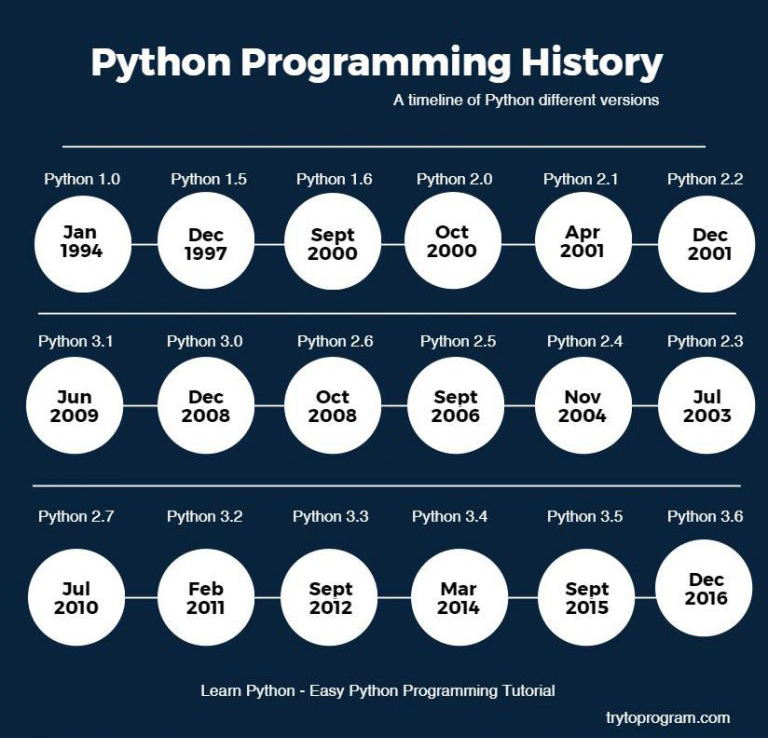
\includegraphics[width=12cm]{pythonhistory} \newline
		Fonte: \url{www.tryprogram.com}
\end{center}
\end{figure}

A seguir \'{e} poss\'{\i}vel observar algumas logotipos da linguagem Python que foram desenvolvidas com o passar dos anos:

\begin{figure}[H]
\begin{center}
	\caption{Logos da Linguagem Python}
	\label{ling2}
	
\includegraphics[width=3cm]{logo1} \quad
	
\includegraphics[width=3cm]{logo2} \quad
	
\includegraphics[width=3cm]{logo3} \newline
	Fonte: \url{www.pngwing.com}
\end{center}
\end{figure}


Dessa forma, conclui-se que o Python \'{e} uma linguagem de programa\c{c}\~{a}o vers\'{a}til e popular que \'{e} utilizada em diversas \'{a}reas, que v\~{a}o desde IA (Intelig\^{e}ncia Artificial) at\'{e} a an\'{a}lise de dados. Como possui uma sintaxe simplista e leg\'{\i}vel a linguagem torna-se f\'{a}cil de aprender e usar, fornecendo aos programadores uma s\'{e}rie de ferramentas e recursos proporcionada pela grande variedade de bibliotecas e estruturas. Como Python est\'{a} se tornando cada vez mais popular provavelmente prosseguir\'{a} a interpretar um papel relevante na \'{a}rea da tecnologia e do software.
  
%%%=========================================================================================%%%
   \section{\'{A}reas de Aplica\c{c}\~{a}o da Linguagem}
%%%=========================================================================================%%%
Python \'{e} uma linguagem de programa\c{c}\~{a}o muito vers\'{a}til que pode ser aplicada em diversas \'{a}reas da tecnologia como, por exemplo big data, orienta\c{c}\~{a}o a objetos, desenvolvimento web e an\'{a}lise de dados.

%%%.........................................................................................%%%
        \subsection{Big Data}
%%%.........................................................................................%%%
De acordo com \cite{McKinney2018}, a linguagem de programa\c{c}\~{a}o Python \'{e} altamente utilizada no campo da big data por possuir a capacidade de tratar uma larga escala de dados e de realizar o processamento paralelo. Al\'{e}m de dispor in\'{u}meras bibliotecas e frameworks para o tratamento de big data ela \'{e} uma linguagem de f\'{a}cil aprendizado.\newline

As principais \'{a}reas de big data em que s\~{a}o utilizados o Python:

\begin{itemize} [itemsep=5pt, parsep=5pt]
\item An\'{a}lise de dados: Python \'{e} utilizado para a an\'{a}lise de dados por dispor in\'{u}meras bibliotecas de an\'{a}lise de dados. As principais utilizadas nessa \'{a}rea s\~{a}o Pandas, NumPy, SciPy, Matplotlib, que possibilitam os desenvolvedores a realizar procedimentos como processamento de dados em larga escala, an\'{a}lise estat\'{\i}stica e visualiza\c{c}\~{a}o de dados.

\item Machine Learning (Aprendizado de M\'{a}quina): Tratando-se de uma das mais utilizadas linguagens de programa\c{c}\~{a}o para a elabora\c{c}\~{a}o de modelos de aprendizado de m\'{a}quina. Python possui TensorFlow, Scikit-learn e PyTorch como bibliotecas famosas de machine learning.

\item Processamento de dados em tempo real: Proporcionando aos programadores um processamento de larga escala de dados e uma resposta mais veloz a eventos em tempo real, as ferramentas como Apache Storm e Apache Kafka s\~{a}o para o processamento de dados em tempo real e amplamente utilizadas em Python.

\item Processamento de dados distribu\'{\i}dos: As ferramentas de sistemas de processamento de dados como Apache Spark e Apache Hadoop de Python possibilitam que programadores processem em larga escala conjuntos de dados em clusters distribu\'{\i}dos de computadores.\newline

\end{itemize} 

Desse modo, devido a possuir uma vasta diversidade de bibliotecas e frameworks, flexibilidade e tamb\'{e}m ser de f\'{a}cil uso, a linguagem de programa\c{c}\~{a}o Python \'{e} uma das principais escolhas para ser utilizada em big data, por existir uma demanda por big data em cont\'{\i}nuo crescimento, Python provavelmente prosseguir\'{a} se tornando uma escolha cada vez mais popular em big data.
        
%%%.........................................................................................%%%		
	\subsection{Orientação a objetos}
%%%.........................................................................................%%%
Entre um mar de linguagens de programa\c{c}\~{a}o orientadas a objetos (POO), o Python, que possui a orienta\c{c}\~{a}o a objetos como parte essencial da linguagem, se destaca fornecendo suporte completo para esse tipo de programa\c{c}\~{a}o. De acordo com \cite{Feltrin2019, Feltrin2020}, a programa\c{c}\~{a}o orientada a objetos \'{e} dedicada \`{a} cria\c{c}\~{a}o de objetos com atributos e m\'{e}todos, organizando-os em classes, hierarquia e heran\c{c}as, servindo assim como um meio de desenvolvimento de software. Al\'{e}m do mais, o Python permite que desenvolvedores criem c\'{o}digos mais modulares e vers\'{a}teis, atrav\'{e}s do polimorfismo em que as classes podem executar o mesmo m\'{e}todo de diferentes maneiras. Ainda, a linguagem de programa\c{c}\~{a}o Python possui uma biblioteca padr\~{a}o poderosa em POO chamada "pickle", que \'{e} utilizada para fazer a desserializa\c{c}\~{a}o e serializa\c{c}\~{a}o de objetos e outra chamada "abc" para definir interfaces e classes abstratas.

Alguns conceitos da orienta\c{c}\~{a}o a objetos em Python:

\begin{itemize} [itemsep=5pt, parsep=5pt]

\item Classes - A classe \'{e} usada para a cria\c{c}\~{a}o de objetos e definir seus m\'{e}todos e atributos.
\subitem Exemplo: A classe chamada 'Pessoa' recebe os atributos: 'nome' e 'idade'.

\item Heran\c{c}a - A heran\c{c}a em Python \'{e} utilizada para a cria\c{c}\~{a}o de novas classes com caracter\'{\i}sticas como atributos e m\'{e}todos, herdadas de classes que j\'{a} existem.
\subitem Exemplo: Uma nova classe 'Faculdade' herda os atributos da classe 'Aluno', podendo ser adicionados novos atributos nessa classe como, 'curso' e 'matr\'{\i}cula'.

\item Hierarquia - Na linguagem de programa\c{c}\~{a}o Python, \'{e} poss\'{\i}vel criar uma hierarquia de classes, ou seja, uma classe \'{e} a "principal" em rela\c{c}\~{a}o a outras classes.
\subitem Exemplo: A classe 'Cachorro' \'{e} a principal em rela\c{c}\~{a}o a classe como 'ra\c{c}a', a qual recebe atributos 'nome' da classe principal, al\'{e}m de ter seus pr\'{o}prios atributos 'cor' e 'porte'.

\item Polimorfismo - Com o polimorfismo \'{e} poss\'{\i}vel criar um m\'{e}todo em uma classe, podendo ser executado de diversas formas.
\subitem Exemplo: Temos a classe 'Pessoa' e outras classes que herdam dela: 'Aluno' e 'Professor', as duas possuem um m\'{e}todo chamado 'matricular' por\'{e}m cada uma implementa de uma forma diferente. \newline

\end{itemize}

Dessa forma, Python \'{e} uma linguagem boa que suporta programa\c{c}\~{a}o orientada a objetos, utilizada frequentemente em desenvolvimento de aplicativos web, desenvolvimentos de jogos, desenvolvimento de aplicativos desktop e etc. Escolhido principalmente por possuir um sintaxe simplista e de f\'{a}cil aprendizagem.
       
%%%.........................................................................................%%%
		\subsection{Desenvolvimento Web}
%%%.........................................................................................%%%
Python \'{e} uma linguagem de programa\c{c}\~{a}o amplamente utilizada no desenvolvimento web, especialmente devido a ter uma vasta diversidade de bibliotecas e frameworks. Os frameworks mais utilizados para o desenvolvimento web s\~{a}o Flask e Django, por\'{e}m existem outros frameworks em Python que s\~{a}o importantes para o desenvolvimento web, como o Pyramid.

De acordo com \cite{BarrosMaciel2020}, os Frameworks em Python utilizados em desenvolvimento web:

\begin{itemize} [itemsep=5pt, parsep=5pt]

\item Django - Um dos frameworks web mais utilizados em Python. Usando o Django criar sites ou aplicativos web escal\'{a}veis e seguros se torna muito f\'{a}cil, pois com ele \'{e} poss\'{\i}vel a cria\c{c}\~{a}o completa desses em pouco tempo, por possuir muitos recursos integrados, como o gerenciamento de URL, autentica\c{c}\~{a}o de usu\'{a}rios e a administra\c{c}\~{a}o de banco de dados.  

\item Flask - Um framework web de aprendizado mais f\'{a}cil que o Django. O Flask \'{e} usado para desenvolver aplica\c{c}\~{o}es web com incomplexidade e rapidez, possuindo como principal caracter\'{\i}stica a facilidade em criar rotas e funcionalidades web.

\item Pyramid - O framework web Pyramid para Python \'{e} o que possui maior flexibilidade e extensividade em rela\c{c}\~{a}o ao Django e ao Flask. Visto que, ele \'{e} apropriado para o desenvolvimento de grandes e complexos aplicativos web, por oferecer autentica\c{c}\~{a}o, cache, seguran\c{c}a e internacionaliza\c{c}\~{a}o que s\~{a}o uma grande diversidade de recursos.  \newline

\end{itemize}

Portanto, a linguagem de programa\c{c}\~{a}o Python \'{e} utilizado em diversas \'{a}reas do desenvolvimento web, que v\~{a}o desde a constru\c{c}\~{a}o de aplicativos web at\'{e} a an\'{a}lise de dados. Python oferece uma grande diversidade de bibliotecas e frameworks que atendem a todas as necessidades de desenvolvimento web, sem depender do tamanho e da dificuldade do projeto.

%%%.........................................................................................%%%        
		\subsection{An\'{a}lise de Dados }
%%%.........................................................................................%%%        
A linguagem Python possui uma diversidade de bibliotecas dispon\'{\i}veis e facilidade de uso tornando-a bem popular em an\'{a}lise de dados - que consiste em coletar, processar e analisar dados para adquirir informa\c{c}\~{o}es relevantes e insights sobre um determinado tema, sendo utilizada em diferentes \'{a}reas, como sa\'{u}de, marketing e finan\c{c}as. As bibliotecas Pandas, NumPy, Matplotlib e SciPy s\~{a}o as mais populares de Python que s\~{a}o empregues nessa \'{a}rea.

De acordo com \cite{McKinney2023, Chen2018}, a an\'{a}lise de dados em Python abrange um conjunto de etapas, a primeira etapa na an\'{a}lise de dados em Python \'{e} coletar os dados relevantes para o problema em quest\~{a}o. Ap\'{o}s realizar a coleta desses dados, \'{e} fundamental prepar\'{a}-los para uma an\'{a}lise. Nesta, \'{e} poss\'{\i}vel ser inclu\'{\i}do o preenchimento de dados ausentes, a limpeza de dados, regulariza\c{c}\~{a}o de dados e a transforma\c{c}\~{a}o desses em formatos apropriados para a an\'{a}lise. Logo ap\'{o}s \'{e} realizado uma an\'{a}lise explorat\'{o}ria de dados (EDA), que \'{e} uma t\'{e}cnica a qual possui como finalidade compreender o grupo de dados, examinando a sua distribui\c{c}\~{a}o, identificando os prov\'{a}veis padr\~{o}es, as tend\^{e}ncias e os v\'{\i}nculos entre as vari\'{a}veis. Al\'{e}m da EDA \'{e} realizada a an\'{a}lise estat\'{\i}stica que \'{e} um procedimento para conhecer as rela\c{c}\~{o}es entre vari\'{a}veis do conjunto de dados. Podendo ser inclu\'{\i}das a an\'{a}lise de correla\c{c}\~{o}es, regress\~{a}o e outras t\'{e}cnicas estat\'{\i}sticas. Ap\'{o}s essas an\'{a}lises, ocorre a modelagem preditiva, que abrange a cria\c{c}\~{a}o de modelos estat\'{\i}sticos para prever efeitos futuros com base nos dados \`{a} disposi\c{c}\~{a}o. A \'{u}ltima etapa da an\'{a}lise de dados em Python realiza a apresenta\c{c}\~{a}o das descobertas da an\'{a}lise de dados de maneira clara e sucinta.

Python em an\'{a}lise de dados realiza um processo iterativo envolvendo diversas etapas, que v\~{a}o desde a coleta de dados at\'{e} o relat\'{o}rio dos resultados. Alguns exemplos de \'{a}reas em que \'{e} largamente usada:

\begin{itemize} [itemsep=5pt, parsep=5pt, topsep=5pt]
  	 	
	\item Finan\c{c}as: Utilizada para realizar a an\'{a}lise de risco, previs\~{a}o de pre\c{c}os e gest\~{a}o de investimentos. 
	
	\item Sa\'{u}de: Usada para prever predisposi\c{c}\~{o}es de sa\'{u}de e reconhecer tratamentos mais eficazes.
	
\end{itemize}

Finda-se ent\~{a}o que a an\'{a}lise de dados em Python est\'{a} em um constante evolu\c{c}\~{a}o, tornando-se poderosa na extra\c{c}\~{a}o de informa\c{c}\~{o}es custosas de um amplo conjunto de dados. Possuindo ferramentas capazes de realizar tarefas desde um simples processamento de dados at\'{e} an\'{a}lises profundas de Machine Learning (Aprendizado de M\'{a}quina).

\chapterimage{capitulo.jpg} % Chapter heading image
% Prof. Dr. Ausberto S. Castro Vera
% UENF - CCT - LCMAT - Curso de Ciência da Computaçãoo
% Campos, RJ,  2023
% Disciplina: Paradigmas de Linguagens de Programação
% Aluno: Mariana Cossetti Dalfior

%%%*****************************************************************************************%%%
\chapter{Conceitos b\'{a}sicos da Linguagem Python}
%%%*****************************************************************************************%%%
Neste cap\'{\i}tulo ser\~{a}o apresentados os aspectos b\'{a}sicos da linguagem de programa\c{c}\~{a}o Python, incluindo atribui\c{c}\~{o}es, vari\'{a}veis, fun\c{c}\~{o}es, estruturas de controle, input/output e tipos de dados.

%%%=========================================================================================%%%
	\section{Vari\'{a}veis}
%%%=========================================================================================%%%
As vari\'{a}veis s\~{a}o elementos essenciais na programa\c{c}\~{a}o em Python, visto que s\~{a}o espa\c{c}os reservados na mem\'{o}ria que armazenam dados - desde n\'{u}mero e textos, at\'{e} objetos - que podem ser alterados durante a execu\c{c}\~{a}o de um programa. Em Python segundo \cite{Sousa2020} as vari\'{a}veis s\~{a}o tratadas como objetos, em que cada objeto receber\'{a} um determinado valor a ser armazenado ou um resultado obtido atrav\'{e}s de um comando. Para a cria\c{c}\~{a}o de uma vari\'{a}vel \'{e} necess\'{a}rio escolher um nome e atribuir a ela uma valor utilizando \textsl{'='}. Exemplos de vari\'{a}veis em Python: 
	
\begin{lstlisting}
>>> # variavel com str
>>> Nome = 'Mariana Cossetti Dalfior'

>>> # variavel com int
>>> Idade = 20

>>> # variavel com float
>>> Peso = 55
\end{lstlisting}

%%%.........................................................................................%%%
		\subsection{Regras de nomenclatura de uma vari\'{a}vel}
%%%.........................................................................................%%%
Existem algumas regras para nomear as vari\'{a}veis em Python. 

O que \'{e} permitido:
	\begin{itemize}
		\item Come\c{c}ar com uma letra ou com um sublinhado '\textsl{\_}'.
		\item O restante do nome pode receber letras, n\'{u}meros e sublinhados.
		\item Os nomes das vari\'{a}veis s\~{a}o sens\'{\i}veis a mai\'{u}sculas e min\'{u}sculas. Ent\~{a}o 'teste' e 'Teste' s\~{a}o nomes distintos de vari\'{a}veis.
	\end{itemize}
		
\begin{lstlisting}
>>> # Permitido
>>> nome
>>> Idade
>>> idade
>>> _bolo
>>> nota_1
\end{lstlisting}
		
		
O que n\~{a}o \'{e} permitidos:
	\begin{itemize}
		\item Come\c{c}ar com n\'{u}mero.
		\item Palavras-chave da linguagem utilizadas para fun\c{c}\~{o}es, como '\textsl{if}', '\textsl{else}', '\textsl{while}', '\textsl{for}', '\textsl{def}', '\textsl{class}' n\~{a}o podem ser empregues como nomes de vari\'{a}veis.
	\end{itemize}
		
\begin{lstlisting}
>>> # Nao permitido
>>> 1bolo
>>> 25_anos
>>> for
>>> %juros
\end{lstlisting}

%%%=========================================================================================%%%
	\section{Constantes}
%%%=========================================================================================%%%
Na linguagem de programa\c{c}\~{a}o Python n\~{a}o existe um tipo espec\'{\i}fico para as constantes como acontece em outras linguagens. Entretanto, de acordo com \cite{Sousa2020} \'{e} poss\'{\i}vel realizar a cria\c{c}\~{a}o de constantes atrav\'{e}s de uma conven\c{c}\~{a}o de nomenclatura, utilizando o nome da constante escrito em letras mai\'{u}sculas e no lugar dos espa\c{c}os utilizar o '\textsl{\_}'. Por\'{e}m, essa conven\c{c}\~{a}o n\~{a}o impossibilita que o valor da vari\'{a}vel seja modificado durante a execu\c{c}\~{a}o do programa, mas faz com que os programadores entendam e tratem essa vari\'{a}vel como constante. Exemplos de constantes em Python:

	
\begin{lstlisting}
>>> # Valor de Pi
>>> PI = 3.141592

>>> # Constante de Napier (base do logaritmo natural)
>>> NAPIER = 2.71828
\end{lstlisting}
	 
Ademais, existem m\'{o}dulos que possuem constantes j\'{a} pr\'{e}-definidas em Python, como o '\textsl{math}' que disp\~{o}em de \textsl{Pi} e a constante de \textsl{Euler}. Como acessar as constantes desse m\'{o}dulo são mostrados a seguir com o c\'{o}digo fonte \ref{fontecons} e o resultado \ref{resulcons} dos exemplos em Python:
	
\begin{lstlisting}
>>> # importando biblioteca
>>> import math
>>>
>>> # mostra pi
>>> print('O valor de Pi: {}' .format(math.pi))
O valor de Pi: 3.41592653589793
>>> 
>>> # mostra euler
>>> print('O valor de Euler: {}' .format(math.e))
O valor de Euler: 2.718281828459045
\end{lstlisting}

\begin{figure}[H]
\begin{center}
	\caption{C\'{o}digo fonte do exemplo de constantes} \label{fontecons}
	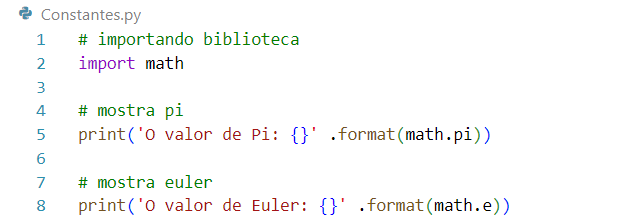
\includegraphics[width=12cm]{constantes} 
	\newline
	Fonte: Criado por Mariana Cossetti Dalfior
\end{center}
\end{figure}

\begin{figure}[H]
\begin{center}
	\caption{Resultado do c\'{o}digo fonte do exemplo de constantes} \label{resulcons}
	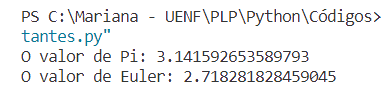
\includegraphics[width=9cm]{resulconstantes} 
	\newline
	Fonte: Criado por Mariana Cossetti Dalfior
\end{center}
\end{figure}

%%%=========================================================================================%%%
	\section{Entrada e Sa\'{\i}da de Dados}
%%%=========================================================================================%%%
Segundo \cite{Yoon2022} a entrada e sa\'{\i}da de dados em Python \'{e} realizada atrav\'{e}s da utiliza\c{c}\~{a}o de uma biblioteca padr\~{a}o.

%%%.........................................................................................%%%
\subsection{Input}
%%%.........................................................................................%%%

A entrada de dados \'{e} feita por meio da fun\c{c}\~{a}o \textsl{'input()'}, permitindo que seja inserido valores ou informa\c{c}\~{o}es - sejam elas strings, n\'{u}meros e  booleanos - pelos usu\'{a}rios enquanto o programa \'{e} executado. Essa fun\c{c}\~{a}o solicita que o usu\'{a}rio digite uma informa\c{c}\~{a}o - a execu\c{c}\~{a}o do programa fica pausada at\'{e} que essa informa\c{c}\~{a}o seja retornada - e ent\~{a}o a armazena em uma vari\'{a}vel. Por\'{e}m todos os dados que s\~{a}o inseridos usando essa fun\c{c}\~{a}o s\~{a}o tratados como strings, ent\~{a}o para transform\'{a}-los em outro tipo ser\'{a} necess\'{a}rio a utiliza\c{c}\~{a}o do \textsl{'int()'} ou \textsl{'float()'}. A seguir \'{e} poss\'{\i}vel observar o c\'{o}digo fonte \ref{fonteinput} e o resultado \ref{resulinput} dos exemplos em Python:

\begin{lstlisting}
>>> # entrada em formato de str
>>> aluno = input('Nome: ')
>>>
>>> # entrada em formato de int
>>> matricula = int(input('Numero de matricula: '))
>>>
>>> # entrada em formato de float
>>> nota = float(input('Nota da prova: '))
>>>
\end{lstlisting}

\begin{figure}[H]
	\begin{center}
		\caption{C\'{o}digo fonte do exemplo de input} \label{fonteinput}
		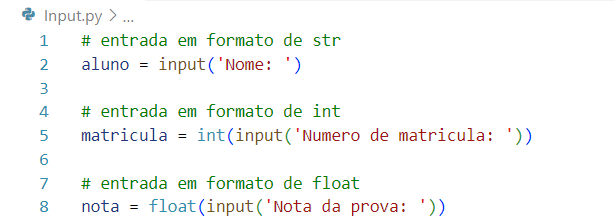
\includegraphics[width=12cm]{input} 
		\newline
		Fonte: Criado por Mariana Cossetti Dalfior
	\end{center}
\end{figure}

\begin{figure}[H]
	\begin{center}
		\caption{Resultado do c\'{o}digo fonte do exemplo de input} \label{resulinput}
		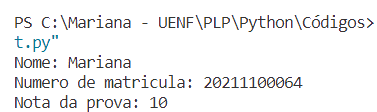
\includegraphics[width=9cm]{resulinput} 
		\newline
		Fonte: Criado por Mariana Cossetti Dalfior
	\end{center}
\end{figure}

%%%.........................................................................................%%%
\subsection{Output}
%%%.........................................................................................%%%

A sa\'{\i}da de dados em Python \'{e} comumente executada pela fun\c{c}\~{a}o \textsl{'print()'}, possuindo como encargo exibir na tela as informa\c{c}\~{a}o geradas pelo programa para o usu\'{a}rio - seja ela uma mensagem, valores e informa\c{c}\~{o}es. EA seguir \'{e} poss\'{\i}vel observar o c\'{o}digo fonte \ref{fontoutput} e o resultado \ref{resuloutput} dos exemplos de sa\'{\i}da de dados em Python:

\begin{lstlisting}
>>> # saida de uma frase
>>> print('Um prato de trigo para tres tigres tristes.')
Um prato de trigo para tres tigres tristes.

>>> # saida do valor de uma variavel
>>> aluno = "Mariana"
>>> matricula = 20211100064
>>> print('{} tem a matricula {}' .format(aluno, matricula))
Mariana tem a matricula 2021110064
\end{lstlisting}

\begin{figure}[H]
	\begin{center}
		\caption{C\'{o}digo fonte do exemplo de output} \label{fonteoutput}
		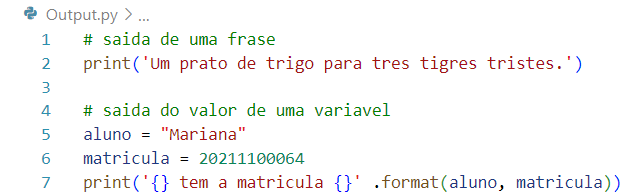
\includegraphics[width=12cm]{output} 
		\newline
		Fonte: Criado por Mariana Cossetti Dalfior
	\end{center}
\end{figure}

\begin{figure}[H]
	\begin{center}
		\caption{Resultado do c\'{o}digo fonte do exemplo de output} \label{resuloutput}
		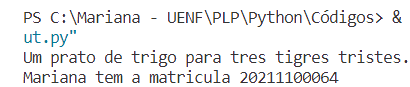
\includegraphics[width=9cm]{resuloutput} 
		\newline
		Fonte: Criado por Mariana Cossetti Dalfior
	\end{center}
\end{figure}
	
No \'{u}ltimo exemplo foi utilizado o \textsl{'format()'}, utilizado para substituir os espa\c{c}os que foram reservados para as vari\'{a}veis fornecidas como argumento.


%%%=========================================================================================%%%
    \section{Tipos de Dados B\'{a}sicos}
%%%=========================================================================================%%%

Os tipos de dados b\'{a}sicos s\~{a}o utilizados para realizar as opera\c{c}\~{o}es b\'{a}sicas de acordo com \cite{Miller2019}. Esses podem ser divididos n\~{a}o seguintes tipos de dados:

%%%.........................................................................................%%%
            \subsection{String} \label{subsec:str}
%%%.........................................................................................%%%
As strings em Python s\~{a}o uma parte fundamental da linguagem, pois representam uma sequ\^{e}ncia de caracteres - podem ser letras, s\'{\i}mbolos, letras e espa\c{c}os em branco. Elas s\~{a}o criadas utilizando aspas simples e duplas. A seguir \'{e} poss\'{\i}vel observar o c\'{o}digo fonte \ref{fontestring} e o resultado \ref{resulstring} dos exemplos de strings em Python:

\begin{lstlisting}
>>> # Usando aspas simples
>>> exemStr = 'Vasco da Gama'
>>> print (exemStr)  
Vasco da Gama

>>> # Usando aspas duplas
>>> exemStr2 = "Vasco da Gama o maior do Rio!"
>>> print (exemStr2)
Vasco da Gama o maior do Rio!
\end{lstlisting}

\begin{figure}[H]
	\begin{center}
		\caption{C\'{o}digo fonte do exemplo de strings} \label{fontestring}
		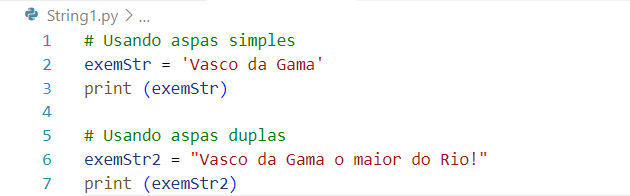
\includegraphics[width=12cm]{string1} 
		\newline
		Fonte: Criado por Mariana Cossetti Dalfior
	\end{center}
\end{figure}

\begin{figure}[H]
	\begin{center}
		\caption{Resultado do c\'{o}digo fonte do exemplo de strings} \label{resulstring}
		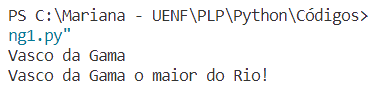
\includegraphics[width=9cm]{resulstring1} 
		\newline
		Fonte: Criado por Mariana Cossetti Dalfior
	\end{center}
\end{figure}

Em Python as strings suportam diversos m\'{e}todos embutidos - que servem para a formata\c{c}\~{a}o e manipula\c{c}\~{a}o das mesmas - como \textsl{'.upper()'} e \textsl{'.lower()'}. A seguir \'{e} poss\'{\i}vel observar o c\'{o}digo fonte \ref{fontestrings2} e o resultado \ref{resulstrings2} dos exemplos de aplica\c{c}\~{a}o desses m\'{e}todos:

\begin{lstlisting}
>>> # Usando o .upper()
>>> exemStr = 'Gabriel Pec'
>>> print(exemStr.upper())
GABRIEL PEC

>>> # Usando o .lower()
>>> exemStr2 = 'Leo Pele'
>>> print(exemStr2.lower())
leo pele
\end{lstlisting}

\begin{figure}[H]
	\begin{center}
		\caption{C\'{o}digo fonte do exemplo de \textsl{.upper} e \textsl{.lower}} \label{fontestrings2}
		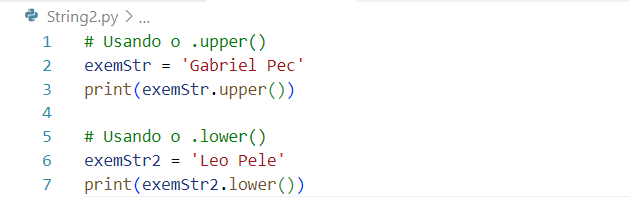
\includegraphics[width=12cm]{string2} 
		\newline
		Fonte: Criado por Mariana Cossetti Dalfior
	\end{center}
\end{figure}

\begin{figure}[H]
	\begin{center}
		\caption{Resultado do c\'{o}digo fonte do exemplo de \textsl{.upper} e \textsl{.lower}} \label{resulstrings2}
		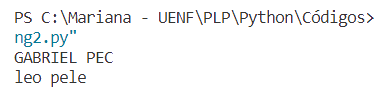
\includegraphics[width=9cm]{resulstring2} 
		\newline
		Fonte: Criado por Mariana Cossetti Dalfior
	\end{center}
\end{figure}

A seguir \'{e} poss\'{\i}vel observar o c\'{o}digo fonte \ref{fonteconcatenacao1}, \ref{fonteconcatenacao2} e o resultado \ref{resulconcatenacao1}, \ref{resulconcatenacao2} dos exemplos de manipula\c{c}\~{a}o de Strings utilizadas em Python:

\begin{itemize}
  \item \textit{Concatena\c{c}\~{a}o de strings}\newline
        Duas ou mais strings podem ser concatenadas utilizando o operador \textsl{'+'}.
        
\begin{lstlisting}
>>> # Concatenando 2 strings
>>> print ("Cruz" + " de Malta")
Cruz de Malta
\end{lstlisting}

\begin{figure}[H]
	\begin{center}
		\caption{C\'{o}digo fonte do exemplo de concatena\c{c}\~{a}o de strings} \label{fonteconcatenacao1}
		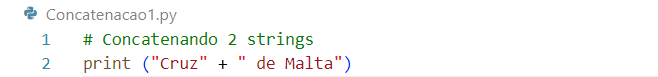
\includegraphics[width=12cm]{concatenacao1} 
		\newline
		Fonte: Criado por Mariana Cossetti Dalfior
	\end{center}
\end{figure}

\begin{figure}[H]
	\begin{center}
		\caption{C\'{o}digo fonte do exemplo de concatena\c{c}\~{a}o de strings} \label{resulconcatenacao1}
		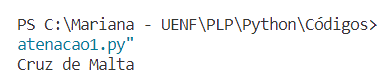
\includegraphics[width=9cm]{resulconcatenacao1} 
		\newline
		Fonte: Criado por Mariana Cossetti Dalfior
	\end{center}
\end{figure}
    
Outra forma de juntar strings e de forma mais eficiente \'{e} atrav\'{e}s do uso do m\'{e}todo \textsl{'.join()'}, capaz de concatenar um lista de strings em apenas uma string.

\begin{lstlisting}
>>> # Concatenando 2 nomes
>>> jogadores = ["Jair", "Andrey"]
>>> print( ", ".join(jogadores))
Jair, Andrey
\end{lstlisting} 

\begin{figure}[H]
	\begin{center}
		\caption{C\'{o}digo fonte do exemplo de concatena\c{c}\~{a}o de lista de strings} \label{fonteconcatenacao2}
		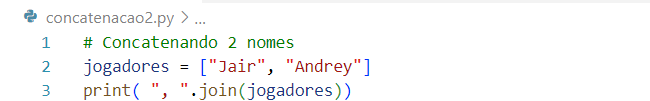
\includegraphics[width=12cm]{concatenacao2} 
		\newline
		Fonte: Criado por Mariana Cossetti Dalfior
	\end{center}
\end{figure}

\begin{figure}[H]
	\begin{center}
		\caption{Resultado do c\'{o}digo fonte do exemplo de concatena\c{c}\~{a}o de lista de strings} \label{resulconcatenacao2}
		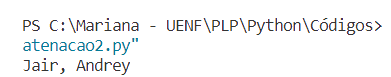
\includegraphics[width=9cm]{resulconcatenacao2} 
		\newline
		Fonte: Criado por Mariana Cossetti Dalfior
	\end{center}
\end{figure}

\item \textit{Operador de indexa\c{c}\~{a}o}\newline
Qualquer elemento individual de uma lista, string ou tupla pode ser acessado com o operador de indexa\c{c}\~{a}o \textsl{'[]'}, usando apenas o \'{\i}ndice entre os colchetes depois da vari\'{a}vel que armazena essa sequ\^{e}ncia. Existem duas formas de indexar os caracteres de um string em Python: \newline
\begin{description}
	  \item[Index com inteiros positivos] come\c{c}ando da esquerda para direita utilizando o 0 como index do primeiro caractere da sequ\^{e}ncia.
	  \item[Index com inteiros negativos] come\c{c}ando da direita para a esquerda utilizando o -1 para iniciar o index sendo ele o \'{u}ltimo elemento da sequ\^{e}ncia, -2 o pen\'{u}ltimo elemento, e assim consecutivamente.
\end{description}

A seguir \'{e} poss\'{\i}vel observar o c\'{o}digo fonte \ref{fontefrase} e o resultado \ref{resulfrase} do exemplo de indexa\c{c}\~{a}o em Python:

\begin{lstlisting}
>>> # indexando com inteiros positivos
>>> frase = "Vasco da Gama"
>>> print(frase[0:5])
Vasco
\end{lstlisting}

\begin{figure}[H]
	\begin{center}
		\caption{C\'{o}digo fonte do exemplo de indexa\c{c}\~{a}o} \label{fontefrase}
		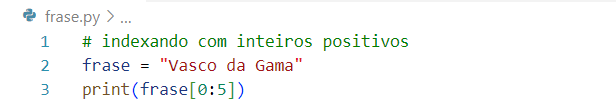
\includegraphics[width=12cm]{frase} 
		\newline
		Fonte: Criado por Mariana Cossetti Dalfior
	\end{center}
\end{figure}

\begin{figure}[H]
	\begin{center}
		\caption{Resultado do c\'{o}digo fonte do exemplo de indexa\c{c}\~{a}o} \label{resulfrase}
		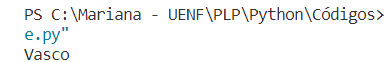
\includegraphics[width=9cm]{resulfrase} 
		\newline
		Fonte: Criado por Mariana Cossetti Dalfior
	\end{center}
\end{figure}

\item \textit{Formata\c{c}\~{a}o de strings}\newline
Strings podem ser formatadas de forma din\^{a}mica com base em valores vari\'{a}veis atrav\'{e}s do m\'{e}todo \textsl{'.format()'}.Esse m\'{e}todo permite a cria\c{c}\~{a}o de strings com espa\c{c}o reservado para serem preenchidos com valores vari\'{a}veis. A seguir \'{e} poss\'{\i}vel observar o c\'{o}digo fonte \ref{fonteformat}, \ref{fonteformat2} e o resultado \ref{resulformat}, \ref{resulformat2} do exemplo da formata\c{c}\~{a}o em Python:
		
\begin{lstlisting}
>>> nome = "Pedro Raul"
>>> idade = 26
>>> print("O jogador {} possui {} anos." .format(nome, idade))
O jogador Pedro Raul possui 26 anos.
\end{lstlisting}
	
\begin{figure}[H]
	\begin{center}
		\caption{C\'{o}digo fonte do exemplo de formata\c{c}\~{a}o de strings} \label{fonteformat}
		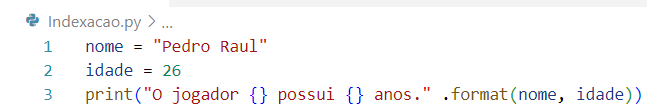
\includegraphics[width=12cm]{format} 
		\newline
		Fonte: Criado por Mariana Cossetti Dalfior
	\end{center}
\end{figure}

\begin{figure}[H]
	\begin{center}
		\caption{Resultado do c\'{o}digo fonte do exemplo de formata\c{c}\~{a}o de strings} \label{resulformat}
		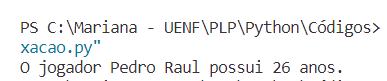
\includegraphics[width=9cm]{resulformat} 
		\newline
		Fonte: Criado por Mariana Cossetti Dalfior
	\end{center}
\end{figure}
	
Em vers\~{o}es mais atuais do Python existe outra tipo de formata\c{c}\~{a}o, utilizando uma forma mais intuitiva e simples. 
		
\begin{lstlisting}
>>> nome = "Pedro Raul"
>>> idade = 26
>>> print("O jogador", nome, "possui", idade, "anos.")
O jogador Pedro Raul possui 26 anos.
\end{lstlisting}

\begin{figure}[H]
	\begin{center}
		\caption{C\'{o}digo fonte do outro exemplo de formata\c{c}\~{a}o de strings} \label{fonteformat2}
		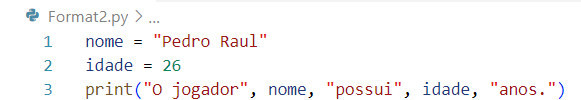
\includegraphics[width=12cm]{format2} 
		\newline
		Fonte: Criado por Mariana Cossetti Dalfior
	\end{center}
\end{figure}

\begin{figure}[H]
	\begin{center}
		\caption{Resultado do c\'{o}digo fonte do outro exemplo de formata\c{c}\~{a}o de strings} \label{resulformat2}
		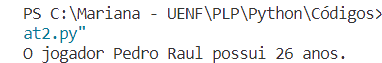
\includegraphics[width=9cm]{resulformat2} 
		\newline
		Fonte: Criado por Mariana Cossetti Dalfior
	\end{center}
\end{figure}
		
    \end{itemize}

%%%.........................................................................................%%%
\subsection{Opera\c{c}\~{o}es l\'{o}gicas}
%%%.........................................................................................%%%
Os operadores l\'{o}gicos s\~{a}o utilizados para realizar opera\c{c}\~{o}es sobre dados booleanos(l\'{o}gicos). Os resultados dessas opera\c{c}\~{o}es podem retornar \textsl{true}(verdadeiro) ou  \textsl{false}(falso). A seguir ser\~{a}o mostrados quais s\~{a}o esses operadores e o que eles significam. \newline

\begin{table}[H]
	\centering
	{\renewcommand\arraystretch{1.25}
		\begin{tabular}{ l l }
			\multicolumn{1}{p{3cm}|} {\centering\textbf{Opera\c{c}\~{o}es}} &
			\multicolumn{1}{p{3cm}}{\centering\textbf{Operador}}
			\\    
			\cline{1-1}\cline{2-2}
			\multicolumn{1}{p{3cm}|}{Menor que} &
			\multicolumn{1}{p{3cm}}{\centering < }
			\\  
			\multicolumn{1}{p{3cm}|}{Maior que} &
			\multicolumn{1}{p{3cm}}{\centering >}
			\\   
			\multicolumn{1}{p{3cm}|}{Menor ou igual} &
			\multicolumn{1}{p{3cm}}{\centering <= }
			\\   
			\multicolumn{1}{p{3cm}|}{Maior ou igual} &
			\multicolumn{1}{p{3cm}}{\centering >=}
			\\   
			\multicolumn{1}{p{3cm}|}{Igual} &
			\multicolumn{1}{p{3cm}}{\centering ==}
			\\   
			\multicolumn{1}{p{3cm}|}{Diferente de} &
			\multicolumn{1}{p{3cm}}{\centering !=}
			\\  
	\end{tabular} }		
	\caption{Opera\c{c}\~{o}es l\'{o}gicas em Python}
\end{table}

A seguir \'{e} poss\'{\i}vel observar o c\'{o}digo fonte \ref{fontelogicas} e o resultado \ref{resullogicas} do exemplo da utiliza\c{c}\~{a}o de opera\c{c}\~{o}es l\'{o}gicas: 
\begin{lstlisting}
	>>> # Menor que
	>>> print(35 < 12)
	False
	>>> # Maior que
	>>> print(64 > 40)
	True
	>>> # Menor ou igual
	>>> print(120 <= 120)
	True
	>>> # Maior ou igual que
	>>> print(32 >= 165)
	False
	>>> # Igual
	>>> print(15 == 80)
	False
	>>> # Diferente de
	>>> print(30 != 15)
	True
\end{lstlisting}

\begin{figure}[H]
	\begin{center}
		\caption{C\'{o}digo fonte do exemplo de opera\c{c}\~{o}es l\'{o}gicas} \label{fontelogicas}
		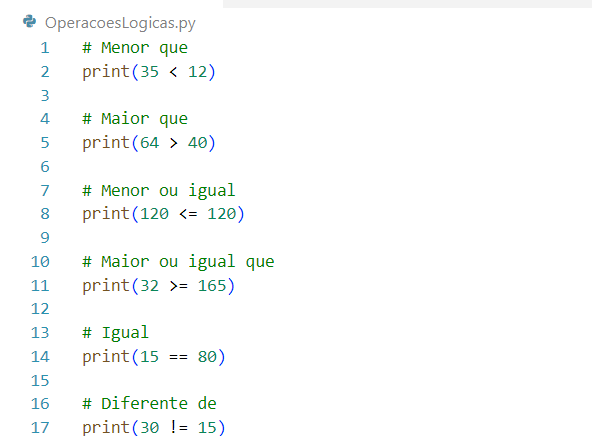
\includegraphics[width=12cm]{logicas} 
		\newline
		Fonte: Criado por Mariana Cossetti Dalfior
	\end{center}
\end{figure}

\begin{figure}[H]
	\begin{center}
		\caption{Resultado do c\'{o}digo fonte do exemplo de opera\c{c}\~{o}es l\'{o}gicas} \label{resullogicas}
		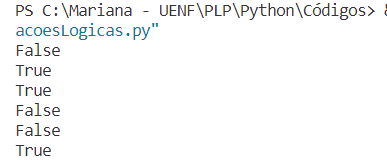
\includegraphics[width=9cm]{resullogicas} 
		\newline
		Fonte: Criado por Mariana Cossetti Dalfior
	\end{center}
\end{figure}

%%%.........................................................................................%%%
		\subsection{N\'{u}meros Inteiros}
%%%.........................................................................................%%%
Os n\'{u}meros inteiros em Python representam todos os n\'{u}meros inteiros positivos, negativos e o zero. Eles s\~{a}o armazenados como objetos inteiros e n\~{a}o possuem limite para o tamanho dos n\'{u}meros que podem ser armazenados em uma vari\'{a}vel inteira. 
Exemplo de n\'{u}mero inteiro em Python:

\begin{lstlisting}
>>> # inteiro positivo
>>> c = 10

>>> # inteiro negativo
>>> r = -200

>>> # zero
>>> v = 0
\end{lstlisting}

Em geral, uma express\~{a}o Python \'{e} uma combina\c{c}\~{a}o de operadores e operandos. Quando avaliamos uma express\~{a}o, obtemos um resultado. Nos pr\'{o}ximos exemplos s\~{a}o realizadas opera\c{c}\~{o}es aritm\'{e}ticas com n\'{u}meros inteiros, como adi\c{c}\~{a}o \textsl{'+'}, subtra\c{c}\~{a}o \textsl{'-'}, multiplica\c{c}\~{a}o \textsl{'*'}, divis\~{a}o \textsl{'/'}, resto da divis\~{a}o \textsl{'\%'} e divis\~{a}o inteira \textsl{'//'} . Ademais, talvez voc\^{e} esteja mais acostumado com \textsl{'x'} e \textsl{'÷'} para multiplica\c{c}\~{a}o e divis\~{a}o, mas em Python e quase todas as outras linguagens de programa\c{c}\~{a}o usam \textsl{'*'} e \textsl{'/'}.  A seguir \'{e} poss\'{\i}vel observar o c\'{o}digo fonte \ref{fonteinteiros} e o resultado \ref{resulinteiros} dos exemplos de n\'{u}mero inteiro em Python:

\begin{lstlisting}
>>> # variaveis 
>>> v = 14
>>> g = 3
>>> 
>>> # soma de inteiros
>>> print(v + g)
17
>>> # subtracao de inteiros
>>> print(v - g) 
11
>>> # multiplicacao de inteiros
>>> print(v * g)
42
>>> # divisao de inteiros
>>> print(v / g)
4.666666666666
>>> # resto da divisao de inteiros
>>> print(v % g)
2
>>> #divisao inteira de inteiros
>>> print(v // g) 
4
\end{lstlisting}

\begin{figure}[H]
	\begin{center}
		\caption{C\'{o}digo fonte do exemplo de opera\c{c}\~{o}es com n\'{u}meros inteiros} \label{fonteinteiros}
		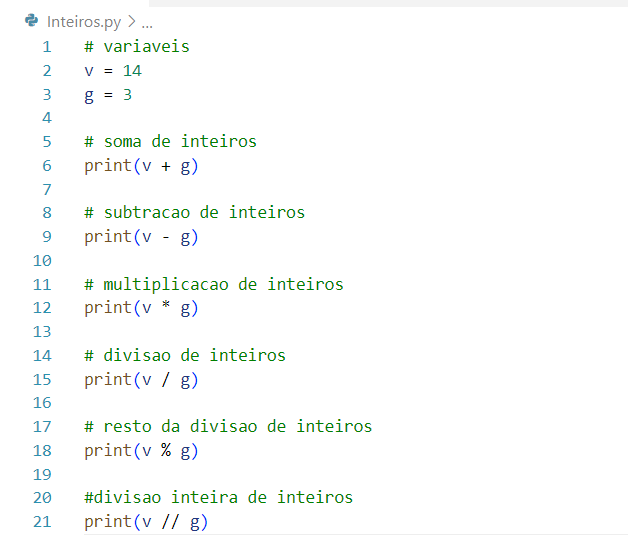
\includegraphics[width=12cm]{inteiros} 
		\newline
		Fonte: Criado por Mariana Cossetti Dalfior
	\end{center}
\end{figure}

\begin{figure}[H]
	\begin{center}
		\caption{Resultado do c\'{o}digo fonte do exemplo de opera\c{c}\~{o}es com n\'{u}meros inteiros} \label{resulinteiros}
		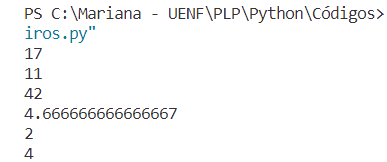
\includegraphics[width=9cm]{resulinteiros} 
		\newline
		Fonte: Criado por Mariana Cossetti Dalfior
	\end{center}
\end{figure}


%%%.........................................................................................%%%
		\subsection{N\'{u}meros de Ponto Flutuante}
%%%.........................................................................................%%%

Os n\'{u}meros de ponto flutuante s\~{a}o a aproxima\c{c}\~{a}o do Python do que voc\^{e} chamou de n\'{u}meros reais nas aula de matem\'{a}tica. Os n\'{u}meros de ponto flutuante s\~{a}o uma aproxima\c{c}\~{a}o porque, diferentemente dos n\'{u}meros reais, os n\'{u}meros de ponto flutuante n\~{a}o podem ter um n\'{u}mero infinito de d\'{\i}gitos ap\'{o}s o ponto decimal. No Python, os n\'{u}meros de ponto flutuante s\~{a}o armazenados como objetos float e s\~{a}o aproximados de forma bin\'{a}ria, podendo apresentar algumas imprecis\~{o}es com valores decimais exatos. A seguir \'{e} poss\'{\i}vel observar o c\'{o}digo fonte \ref{fontefloat1} e o resultado \ref{resulfloat1} do exemplo de n\'{u}meros de ponto flutuante em Python:

\begin{lstlisting}
>>> # variaveis
>>> v = 0.5
>>> g = 0.2
>>> # soma de floats
>>> f = v + g
>>> print(f)
0.7
\end{lstlisting}

\begin{figure}[H]
	\begin{center}
		\caption{C\'{o}digo fonte do exemplo com n\'{u}meros de ponto flutuante} \label{fontefloat1}
		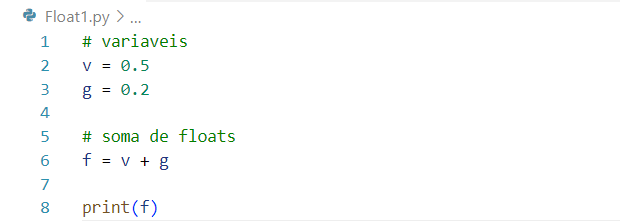
\includegraphics[width=12cm]{float1} 
		\newline
		Fonte: Criado por Mariana Cossetti Dalfior
	\end{center}
\end{figure}

\begin{figure}[H]
	\begin{center}
		\caption{Resultado do c\'{o}digo fonte do exemplo com n\'{u}meros de ponto flutuante} \label{resulfloat1}
		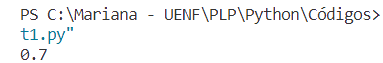
\includegraphics[width=9cm]{resulfloat1} 
		\newline
		Fonte: Criado por Mariana Cossetti Dalfior
	\end{center}
\end{figure}

Do mesmo modo que os n\'{u}meros inteiros, \'{e} poss\'{\i}vel realizar opera\c{c}\~{o}es aritm\'{e}ticas com n\'{u}meros de ponto flutuante, como adi\c{c}\~{a}o \textsl{'+'}, subtra\c{c}\~{a}o \textsl{'-'}, multiplica\c{c}\~{a}o \textsl{'*'}, divis\~{a}o \textsl{'/'}, resto da divis\~{a}o \textsl{'\%'} e divis\~{a}o inteira \textsl{'//'}. A seguir \'{e} poss\'{\i}vel observar o c\'{o}digo fonte \ref{fontefloat2} e o resultado \ref{resulfloat2} do exemplo de opera\c{c}\~{o}es aritm\'{e}ticas com n\'{u}meros de ponto flutuante em Python:

\begin{lstlisting}
>>> # variaveis 
>>> v = 10.33
>>> g = 5
>>>
>>> # soma de floats
>>> print(v + g)
15.33
>>> # subtracao de floats
>>> print(v - g) 
5.33
>>> # multiplicacao de floats
>>> print(v * g)
51.65
>>> # divisao de floats
>>> print(v / g)
2.066
>>> # resto da divisao de floats
>>> print(v % g)
0.3300000000007
>>> #divisao inteira de floats
>>> print(v // g) 
2.0
\end{lstlisting}

\begin{figure}[H]
	\begin{center}
		\caption{C\'{o}digo fonte do exemplo de opera\c{c}\~{o}es com n\'{u}meros de ponto flutuante} \label{fontefloat2}
		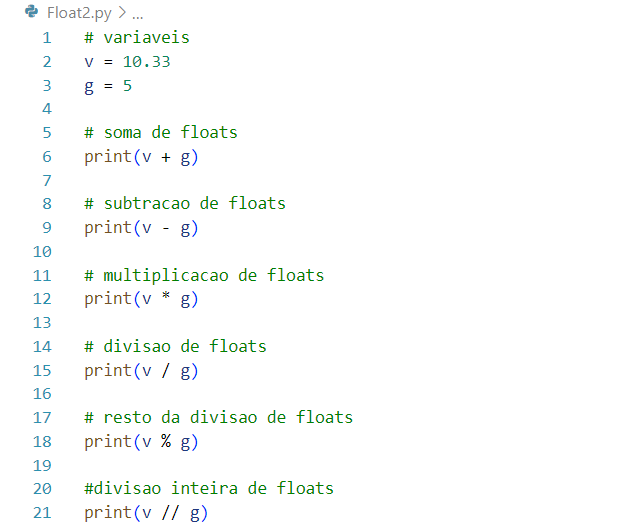
\includegraphics[width=12cm]{float2} 
		\newline
		Fonte: Criado por Mariana Cossetti Dalfior
	\end{center}
\end{figure}

\begin{figure}[H]
	\begin{center}
		\caption{Resultado do c\'{o}digo fonte do exemplo de opera\c{c}\~{o}es com n\'{u}meros de ponto flutuante} \label{resulfloat2}
		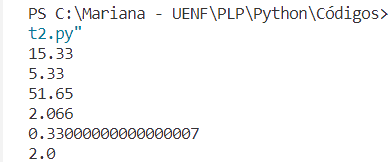
\includegraphics[width=9cm]{resulfloat2} 
		\newline
		Fonte: Criado por Mariana Cossetti Dalfior
	\end{center}
\end{figure}

%%%.........................................................................................%%%
\subsection{N\'{u}meros complexos}
%%%.........................................................................................%%%

O \'{u}ltimo tipo num\'{e}rico primitivo em Python \'{e} o n\'{u}mero complexo. Como voc\^{e} pode se recordar, os n\'{u}meros complexos t\^{e}m duas partes: uma parte real e uma parte imagin\'{a}ria. No Python, um n\'{u}mero complexo \'{e} exibido como \textsl{real} + \textsl{imagin\'{a}rio}j. A seguir \'{e} poss\'{\i}vel observar o c\'{o}digo fonte \ref{fontecomplexos} e o resultado \ref{resulcomplexos} do exemplo de n\'{u}meros complexos em Python:

\begin{lstlisting}
>>> # Numeros complexos
>>> print(100000000000000000000000000 * 3.4)
3.40000000000000003e+26 
>>> print(5 + 4+3j)
(9 + 3j)
>>>
\end{lstlisting}

\begin{figure}[H]
	\begin{center}
		\caption{C\'{o}digo fonte do exemplo com n\'{u}meros complexos} \label{fontecomplexos}
		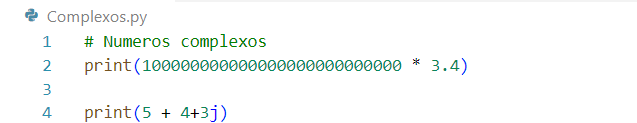
\includegraphics[width=12cm]{complexos} 
		\newline
		Fonte: Criado por Mariana Cossetti Dalfior
	\end{center}
\end{figure}

\begin{figure}[H]
	\begin{center}
		\caption{Resultado do c\'{o}digo fonte do exemplo com n\'{u}meros complexos} \label{resulcomplexos}
		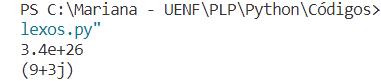
\includegraphics[width=9cm]{resulcomplexos} 
		\newline
		Fonte: Criado por Mariana Cossetti Dalfior
	\end{center}
\end{figure}


%%%.........................................................................................%%%
		\subsection{Booleanos}
%%%.........................................................................................%%%
 Os booleanos s\~{a}o escritos como palavras-chave '\textsl{True}' e '\textsl{False}', sem aspas e com a primeira letra em mai\'{u}scula. S\~{a}o utilizados em express\~{o}es l\'{o}gicas e em estruturas de controle de fluxo, como o \textsl{if} e o \textsl{while}, podendo ser combinados com o \textsl{and}, \textsl{or} e \textsl{not}. A seguir \'{e} poss\'{\i}vel observar o c\'{o}digo fonte \ref{fontebool} e o resultado \ref{resulbool} do exemplo de booleano usado em um \textsl{if} com \textsl{and} :

\begin{lstlisting}
>>> # variaveis
>>> v = 6
>>> g = 12
>>> 
>>> if v > 5 and g > 3:
>>> 	print("{} maior que 5 e {} e maior que 3" .format(v, g))
6 e maior que 5 e 12 maior que 3
\end{lstlisting}

\begin{figure}[H]
	\begin{center}
		\caption{C\'{o}digo fonte do exemplo com n\'{u}meros booleanos em um \textsl{if}} \label{fontebool}
		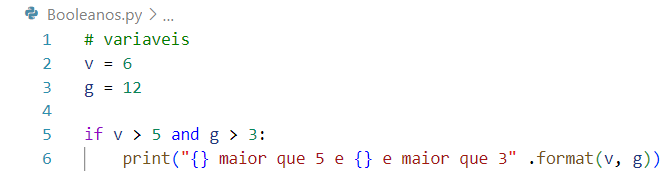
\includegraphics[width=12cm]{bool} 
		\newline
		Fonte: Criado por Mariana Cossetti Dalfior
	\end{center}
\end{figure}

\begin{figure}[H]
	\begin{center}
		\caption{Resultado do c\'{o}digo fonte do exemplo com n\'{u}meros booleanos em um \textsl{if}} \label{resulbool}
		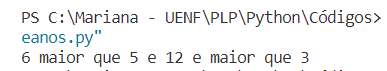
\includegraphics[width=9cm]{resulbool} 
		\newline
		Fonte: Criado por Mariana Cossetti Dalfior
	\end{center}
\end{figure}

Ademais,  \'{e} poss\'{\i}vel converter qualquer valor ou express\~{a}o em um booleano utilizando uma fun\c{c}\~{a}o chamada \textsl{'bool()'}.Essa fun\c{c}\~{a}o retorna '\textsl{False}' caso o valor for considerado "vazio", e '\textsl{True}' caso contr\'{a}rio. A seguir \'{e} poss\'{\i}vel observar o c\'{o}digo fonte \ref{fontebool2} e o resultado \ref{resulbool2} do exemplo: 

\begin{lstlisting}
>>> print(bool(0))       
False
>>> print(bool(1898))       
True
>>> print(bool(""))      
False
>>> print(bool("Vasco")) 
True
\end{lstlisting}

\begin{figure}[H]
	\begin{center}
		\caption{C\'{o}digo fonte do exemplo com n\'{u}meros booleanos} \label{fontebool2}
		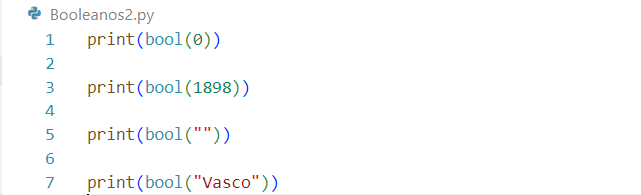
\includegraphics[width=12cm]{bool2} 
		\newline
		Fonte: Criado por Mariana Cossetti Dalfior
	\end{center}
\end{figure}

\begin{figure}[H]
	\begin{center}
		\caption{Resultado do c\'{o}digo fonte do exemplo com n\'{u}meros booleanos} \label{resulbool2}
		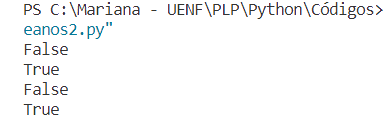
\includegraphics[width=9cm]{resulbool2} 
		\newline
		Fonte: Criado por Mariana Cossetti Dalfior
	\end{center}
\end{figure}

Em resumo, foi evidenciado que o Python oferece suporte a v\'{a}rios tipos diferentes de objetos primitivos: n\'{u}meros inteiros, n\'{u}meros de ponto flutuante, n\'{u}meros complexos, n\'{u}meros booleanos, Strings e as opera\c{c}\~{o}es l\'{o}gicas.

%%%=========================================================================================%%%
    \section{Estrutura de Controle e Fun\c{c}\~{o}es}
%%%=========================================================================================%%%
As estruturas de controle e fun\c{c}\~{o}es s\~{a}o elementos fundamentais da programa\c{c}\~{a}o em Python. A seguir ser\~{a}o mostradas algumas dessas estruturas segundo \cite{Guttag2021}: 
%%%.........................................................................................%%%
            \subsection{O comando \textsl{If}}
%%%.........................................................................................%%%
O comando "\textsl{if}" em Python \'{e} uma estrutura de controle que permite executar determinado bloco de c\'{o}digo se uma determinada condi\c{c}\~{a}o for verdadeira. A sintaxe b\'{a}sica em Python \'{e} a seguinte:
\begin{lstlisting}
>>> if condicao:
>>> 	# bloco de codigo
\end{lstlisting}	

A seguir \'{e} poss\'{\i}vel observar o c\'{o}digo fonte \ref{fonteif} e o resultado \ref{resulif} do exemplo com aplica\c{c}\~{a}o em Python:

\begin{lstlisting}
>>> # variavel
>>> v = 10
>>> 
>>> if v > 5:
>>> 	print("Gigante da Colina")
Gigante da Colina
\end{lstlisting}	

\begin{figure}[H]
	\begin{center}
		\caption{C\'{o}digo fonte do exemplo do uso do \textsl{if}} \label{fonteif}
		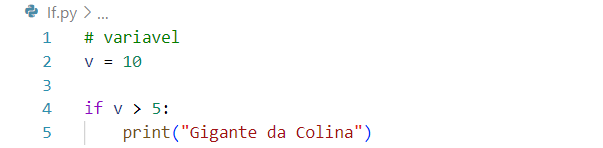
\includegraphics[width=12cm]{if} 
		\newline
		Fonte: Criado por Mariana Cossetti Dalfior
	\end{center}
\end{figure}

\begin{figure}[H]
	\begin{center}
		\caption{Resultado do c\'{o}digo fonte do exemplo do uso do \textsl{if}} \label{resulif}
		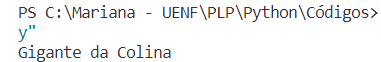
\includegraphics[width=9cm]{resulif} 
		\newline
		Fonte: Criado por Mariana Cossetti Dalfior
	\end{center}
\end{figure}
%%%.........................................................................................%%%
			\subsection{O comando \textsl{Else}}
%%%.........................................................................................%%%
O comando '\textsl{else}' \'{e} sempre utilizado em conjunto com o '\textsl{if}' para fornecer uma alternativa caso a condi\c{c}\~{a}o do \textsl{if} n\~{a}o seja verdadeira. Dessa forma, o bloco de c\'{o}digo dentro do \textsl{else} s\'{o} ser\'{a} executado se a condi\c{c}\~{a}o do \textsl{if} for falsa. A sintaxe b\'{a}sica em Python \'{e} a seguinte:
\begin{lstlisting}
>>> if condicao:
>>> 	# bloco de codigo a ser executado se a condicao for 
>>> 	# verdadeira
>>> else:
>>> 	# bloco de codigo a ser executado se a condicao for 
>>> 	# falsa
\end{lstlisting}	

A seguir \'{e} poss\'{\i}vel observar o c\'{o}digo fonte \ref{fonteelse} e o resultado \ref{resulelse} do exemplo com aplica\c{c}\~{a}o em Python:

\begin{lstlisting}
>>> # variavel
>>> v = 12
>>>
>>> if v % 2 == 0:
>>> 	print("O numero e par")
>>> else:
>>> 	print("O numero e impar")
O numero e par
\end{lstlisting}	

\begin{figure}[H]
\begin{center}
	\caption{C\'{o}digo fonte do exemplo do uso do \textsl{else}} \label{fonteelse}
	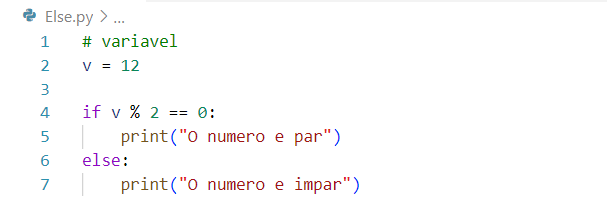
\includegraphics[width=12cm]{else} 
	\newline
	Fonte: Criado por Mariana Cossetti Dalfior
\end{center}
\end{figure}

\begin{figure}[H]
\begin{center}
	\caption{Resultado do c\'{o}digo fonte do exemplo do uso do \textsl{else}} \label{resulelse}
	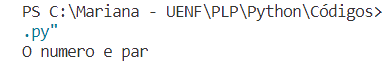
\includegraphics[width=9cm]{resulelse} 
	\newline
	Fonte: Criado por Mariana Cossetti Dalfior
\end{center}
\end{figure}

%%%.........................................................................................%%%
			\subsection{O comando \textsl{Elif}}
%%%.........................................................................................%%%
O comando "\textsl{elif} " - abrevia\c{c}\~{a}o de "\textsl{else} "  e "\textsl{if} "  - \'{e} utilizado para adicionar uma condi\c{c}\~{a}o adicional a um bloco \textsl{if-else}. Normalmente usado quando existem mais de duas condi\c{c}\~{o}es poss\'{\i}veis que precisam ser avaliadas. Se a condi\c{c}\~{a}o do \textsl{if} n\~{a}o for atendida, o programa passar\'{a} para a pr\'{o}xima condi\c{c}\~{a}o \textsl{elif}. Se nenhuma das condi\c{c}\~{o}es \textsl{if} ou \textsl{elif} for atendida, o bloco \textsl{else} final ser\'{a} executado. A sintaxe do comando \textsl{elif} em Python \'{e} a seguinte: \newline

\begin{lstlisting}
>>> if condicao1:
>>> 	# Bloco de codigo se condicao1 for verdadeira
>>> elif condicao2:
>>> 	# Bloco de codigo se condicao2 for verdadeira
>>> elif condicao3:
>>> 	# Bloco de codigo se condicao3 for verdadeira
>>> ...
>>> else:
>>> 	# Bloco de codigo se nenhuma das condicoes anteriores 
>>> 	for verdadeira
\end{lstlisting}	

A seguir \'{e} poss\'{\i}vel observar o c\'{o}digo fonte \ref{fonteelif} e o resultado \ref{resulelif} do exemplo com aplica\c{c}\~{a}o em Python:

\begin{lstlisting}
>>> # variavel
>>> idade = 20
>>> 
>>> if idade < 18:
>>> 	print("Voce e menor de idade")
>>> elif idade >= 18 and idade < 65:
>>> 	print("Voce e adulto")
>>> else:
>>> 	print("Voce e idoso")
voce e adulto
\end{lstlisting}	

\begin{figure}[H]
	\begin{center}
		\caption{C\'{o}digo fonte do exemplo do uso do \textsl{elif}} \label{fonteelif}
		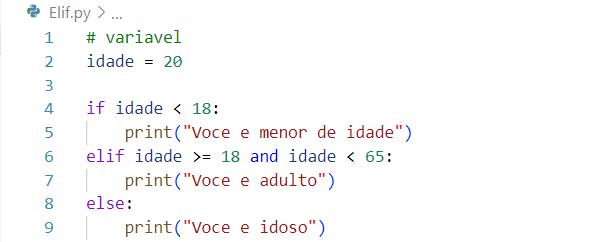
\includegraphics[width=12cm]{elif} 
		\newline
		Fonte: Criado por Mariana Cossetti Dalfior
	\end{center}
\end{figure}

\begin{figure}[H]
	\begin{center}
		\caption{Resultado do c\'{o}digo fonte do exemplo do uso do \textsl{elif}} \label{resulelif}
		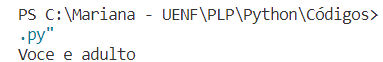
\includegraphics[width=9cm]{resulelif} 
		\newline
		Fonte: Criado por Mariana Cossetti Dalfior
	\end{center}
\end{figure}

%%%.........................................................................................%%%
            \subsection{La\c{c}o \textsl{For}}
%%%.........................................................................................%%%
O la\c{c}o "\textsl" \'{e} usado para iterar sobre uma sequ\^{e}ncia, sendo uma estrutura de controle de fluxo que repete um bloco de c\'{o}digo um determinado n\'{u}mero de vezes, at\'{e} atingir a condi\c{c}\~{a}o de parada. Al\'{e}m de que \'{e} poss\'{\i}vel combinar o \textsl{for} com outros comandos, como \textsl{if}, \textsl{else}, \textsl{break} e \textsl{continue}, para criar l\'{o}gicas mais complexas dentro do la\c{c}o. A sintaxe b\'{a}sica do la\c{c}o \textsl{for} em Python \'{e} a seguinte:

\begin{lstlisting}
>>> for <variavel> in <sequencia>:
>>> # bloco de codigo
\end{lstlisting}	

Durante cada itera\c{c}\~{a}o do la\c{c}o \textsl{for}, a vari\'{a}vel de itera\c{c}\~{a}o vai sendo incrementada, e o bloco de c\'{o}digo \'{e} executado com esse valor. O la\c{c}o continua at\'{e} que todos os itens da sequ\^{e}ncia tenham sido processados. A seguir \'{e} poss\'{\i}vel observar o c\'{o}digo fonte \ref{fontefor} e o resultado \ref{resulfor} do exemplo de um \textsl{for} em Python:

\begin{lstlisting}
>>> lista = [1, 2, 3, 4, 5]
>>> for v in lista:
>>> 	print(v)
1
2 
3
4
5
\end{lstlisting}	

\begin{figure}[H]
	\begin{center}
		\caption{C\'{o}digo fonte do exemplo do uso do \textsl{for}} \label{fontefor}
		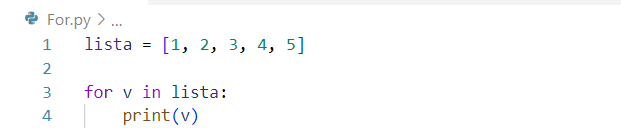
\includegraphics[width=12cm]{for} 
		\newline
		Fonte: Criado por Mariana Cossetti Dalfior
	\end{center}
\end{figure}

\begin{figure}[H]
	\begin{center}
		\caption{Resultado do c\'{o}digo fonte do exemplo do uso do \textsl{for}} \label{resulfor}
		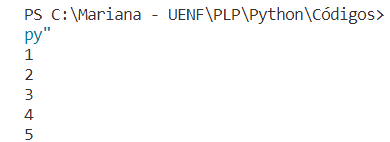
\includegraphics[width=9cm]{resulfor} 
		\newline
		Fonte: Criado por Mariana Cossetti Dalfior
	\end{center}
\end{figure}

%%%.........................................................................................%%%
            \subsection{La\c{c}o \textsl{While}}
%%%.........................................................................................%%%
O la\c{c}o de repeti\c{c}\~{a}o "\textsl{while}" \'{e} utilizado para repetir um bloco de c\'{o}digo at\'{e} uma condi\c{c}\~{a}o for falsa. A sua sintaxe geral em Python \'{e} a seguinte:

\begin{lstlisting}
>>> while condicao:
>>> # bloco de codigo a ser executado enquanto a condicao for 
>>> # verdadeira
\end{lstlisting}	

O bloco de c\'{o}digo dentro do la\c{c}o \textsl{while} vai ser executado diversas vezes at\'{e} que a condi\c{c}\~{a}o seja falsa. \'{E} necess\'{a}rio ter bastante cuidado para evitar a cria\c{c}\~{a}o de um loop infinito, pois a condi\c{c}\~{a}o nunca se torna falsa e ent\~{a}o o programa nunca parar\'{a} de ser executado. A seguir \'{e} poss\'{\i}vel observar o c\'{o}digo fonte \ref{fontewhile} e o resultado \ref{resulwhile} do exemplo de um laço \textsl{while} em Python:

\begin{lstlisting}
>>> # variaveis
>>> soma = 0
>>> v = 1
>>> 
>>> while v <= 10:
>>> 	soma += v
>>> 	v += 1
>>> print(soma)
55
\end{lstlisting}	

\begin{figure}[H]
	\begin{center}
		\caption{C\'{o}digo fonte do exemplo do uso do \textsl{while}} \label{fontewhile}
		\includegraphics[width=12cm]{while} 
		\newline
		Fonte: Criado por Mariana Cossetti Dalfior
	\end{center}
\end{figure}

\begin{figure}[H]
	\begin{center}
		\caption{Resultado do c\'{o}digo fonte do exemplo do uso do \textsl{while}} \label{resulwhile}
		\includegraphics[width=9cm]{resulwhile} 
		\newline
		Fonte: Criado por Mariana Cossetti Dalfior
	\end{center}
\end{figure}
% Prof. Dr. Ausberto S. Castro Vera
% UENF - CCT - LCMAT - Curso de Ci\^{e}ncia da Computa\c{c}\~{a}o
% Campos, RJ,  2023
% Disciplina: Paradigmas de Linguagens de Programa\c{c}\~{a}o
% Aluno: Mariana Cossetti Dalfior

%%%*****************************************************************************************%%%
\chapter{Aspectos Avan\c{c}ados da Linguagem Python}
%%%*****************************************************************************************%%%
Neste cap\'{\i}tulo ser\~{a}o apresentados os aspectos avan\c{c}ados da linguagem de programa\c{c}\~{a}o Python, incluindo classes, dados de cole\c{c}\~{a}o e fun\c{c}\~{o}es geradoras.

%%%=========================================================================================%%%
\section{Classes}
%%%=========================================================================================%%%
De acordo com \cite{Ramalho2022} Python oferece algumas maneiras de construir uma classe simples que \'{e} apenas uma cole\c{c}\~{a}o de campos, com pouca ou nenhuma funcionalidade extra. Esse padr\~{a}o \'{e} conhecido como \textquotedblleft{}classe de dados\textquotedblright{} \textemdash{} e as classes de dados s\~{a}o um dos pacotes que suportam esse padr\~{a}o.

%%%.........................................................................................%%%		
	\subsection{Classes base Abstratas}
%%%.........................................................................................%%%
As classes abstratas podem ser utilizadas do m\'{o}dulo \textsl{collections.abc} como \textsl{Mapping} e \textsl{MutableMapping}. Idealmente, uma fun\c{c}\~{a}o deve aceitar argumentos desses tipos abstratos e n\~{a}o tipos concretos. Isso d\'{a} mais flexibilidade ao chamador. Considere esta assinatura de fun\c{c}\~{a}o:

\begin{lstlisting}
>>> # Usar abc.Mapping permite que o chamador forneca uma 
>>> # instancia de dict, defaultdict, ChainMap, uma subclasse 
>>> # UserDict ou qualquer outro tipo que seja um subtipo 
>>> # de Mapping.
>>>
>>> from collections.abc import Mapping
>>> def nome2hex(nome: str, color_map: Mapeamento[str, int]) -> str:
\end{lstlisting}

%%%=========================================================================================%%%
\section{Tipos de Dados de Cole\c{c}\~{a}o}
%%%=========================================================================================%%%
Os tipos de dados de cole\c{c}\~{a}o s\~{a}o utilizados para guardar cole\c{c}\~{o}es de valores de acordo com \cite{Perkovic2016}. Esses podem ser divididos em dois: tipos sequenciais e tipos conjuntos.
%%%.........................................................................................%%%
\subsection{Tipos Sequenciais}
%%%.........................................................................................%%%
Os tipos sequenciais s\~{a}o utilizados para armazenar dados em sequ\^{e}ncia, ou seja, em uma ordem espec\'{\i}fica. Existem tr\^{e}s tipos de sequ\^{e}ncia em Python, as listas, tuplas e strings (exibido anteriormente nesse cap\'{\i}tulo em \ref{subsec:str}):				

%%%¨¨¨¨¨¨¨¨¨¨¨¨¨¨¨¨¨¨¨¨¨¨¨¨¨¨¨¨¨¨¨¨¨¨¨¨¨¨¨¨¨¨¨¨¨¨¨¨¨¨¨¨¨¨¨¨¨¨¨¨¨¨¨¨¨¨¨¨¨¨¨¨¨¨¨¨¨¨¨¨¨¨¨¨¨¨¨¨¨%%%
\subsubsection{Listas} \label{cap3/3.2.1}
%%%¨¨¨¨¨¨¨¨¨¨¨¨¨¨¨¨¨¨¨¨¨¨¨¨¨¨¨¨¨¨¨¨¨¨¨¨¨¨¨¨¨¨¨¨¨¨¨¨¨¨¨¨¨¨¨¨¨¨¨¨¨¨¨¨¨¨¨¨¨¨¨¨¨¨¨¨¨¨¨¨¨¨¨¨¨¨¨¨¨%%%
As listas s\~{a}o cole\c{c}\~{o}es ordenadas de elementos que podem ser de diferentes tipos de dados - como inteiros, strings, booleanos e at\'{e} outras listas. Elas s\~{a}o uma das estruturas mais utilizadas em Python por serem muito vers\'{a}teis - podendo ser modificadas removendo, alterando e adicionando novos elementos ap\'{o}s a sua cria\c{c}\~{a}o. As listas s\~{a}o criadas utilizando \textsl{'[]'} e seus elementos s\~{a}o separados por v\'{\i}rgulas e indexados de forma num\'{e}rica - inicia com \'{\i}ndice 0 para o primeiro elemento e vai aumentando de um em um para os \'{\i}ndices posteriores. A seguir \'{e} poss\'{\i}vel observar o c\'{o}digo fonte \ref{fontelistas1} e o resultado \ref{resullistas1} do exemplo da utiliza\c{c}\~{a}o de listas em Python:

\begin{lstlisting}
>>> # utilizando apenas numeros inteiros
>>> num = [1, 2, 3, 4, 5]
>>> print(num[4])
5

>>> # utilizando apenas strings 
>>> vasco = ["Andrey", "Puma", "Pedro Raul"]
>>> print(vasco[1])
Puma

>>> # utilizando de forma mista
>>> junto = [7, "Piton", 5.0, False]
>>> print(junto[3])
False
\end{lstlisting}

\begin{figure}[H]
	\begin{center}
		\caption{C\'{o}digo fonte do exemplo do uso listas} \label{fontelistas1}
		\includegraphics[width=12cm]{listas1} 
		\newline
		Fonte: Criado por Mariana Cossetti Dalfior
	\end{center}
\end{figure}

\begin{figure}[H]
	\begin{center}
		\caption{Resultado do c\'{o}digo fonte do exemplo do uso listas} \label{resullistas1}
		\includegraphics[width=9cm]{resullistas1} 
		\newline
		Fonte: Criado por Mariana Cossetti Dalfior
	\end{center}
\end{figure}

\'{E} poss\'{\i}vel realizar opera\c{c}\~{o}es comuns nas listas utilizando os m\'{e}todos, como \textsl{'.append()'}, \textsl{'.extend()'}, \textsl{'.insert()'}, \textsl{'.remove()'}, \textsl{'.pop()'}, \textsl{'.index()'}, \textsl{'.count()'} e \textsl{'.sort()'}. A seguir \'{e} poss\'{\i}vel observar o c\'{o}digo fonte \ref{fontelistas2} e o resultado \ref{resullistas2} do exemplo da utiliza\c{c}\~{a}o de m\'{e}todos em listas:

\begin{lstlisting}
>>> # utilizando append
>>> num = [1, 2, 3, 4, 5]
>>> num.append(6)
>>> print(num)
[1, 2, 3, 4, 5, 6]

>>> # utilizando extend 
>>> num = [2, 4, 6]
>>> impares = [1, 3, 5]
>>> num.extend(impares)
>>> print(num)
[1, 2, 3, 4, 5, 6]

>>> # utilizando insert
>>> num = [1, 2, 3, 4, 5]
>>> num.insert(1, 'Vasco')
>>> print(num)
[1, 'Vasco', 2, 3, 4, 5]
	
\end{lstlisting}

\begin{figure}[H]
	\begin{center}
		\caption{C\'{o}digo fonte do exemplo da utiliza\c{c}\~{a}o de m\'{e}todos em listas} \label{fontelistas2}
		\includegraphics[width=12cm]{listas2} 
		\newline
		Fonte: Criado por Mariana Cossetti Dalfior
	\end{center}
\end{figure}

\begin{figure}[H]
	\begin{center}
		\caption{Resultado do c\'{o}digo fonte do exemplo da utiliza\c{c}\~{a}o de m\'{e}todos em listas} \label{resullistas2}
		\includegraphics[width=9cm]{resullistas2} 
		\newline
		Fonte: Criado por Mariana Cossetti Dalfior
	\end{center}
\end{figure}

%%%¨¨¨¨¨¨¨¨¨¨¨¨¨¨¨¨¨¨¨¨¨¨¨¨¨¨¨¨¨¨¨¨¨¨¨¨¨¨¨¨¨¨¨¨¨¨¨¨¨¨¨¨¨¨¨¨¨¨¨¨¨¨¨¨¨¨¨¨¨¨¨¨¨¨¨¨¨¨¨¨¨¨¨¨¨¨¨¨¨%%%
\subsubsection{Tuplas}
%%%¨¨¨¨¨¨¨¨¨¨¨¨¨¨¨¨¨¨¨¨¨¨¨¨¨¨¨¨¨¨¨¨¨¨¨¨¨¨¨¨¨¨¨¨¨¨¨¨¨¨¨¨¨¨¨¨¨¨¨¨¨¨¨¨¨¨¨¨¨¨¨¨¨¨¨¨¨¨¨¨¨¨¨¨¨¨¨¨¨%%%
As tuplas s\~{a}o um tipo de dado de cole\c{c}\~{a}o, parecidos com as listas, diferente delas possui como caracter\'{\i}sticas serem imut\'{a}veis - n\~{a}o podem ser modificadas depois de sua cria\c{c}\~{a}o. Al\'{e}m disso, elas geralmente s\~{a}o usadas para o armazenamento de dados que s\~{a}o relacionados, diferente das listas que s\~{a}o utilizadas para armazenar cole\c{c}\~{o}es de objetos. As tuplas s\~{a}o criadas de diversas maneiras em Python, por\'{e}m a mais comum \'{e} utilizando par\^{e}nteses \textsl{'()'}. Exemplo da utiliza\c{c}\~{a}o de tuplas em Python: 

\begin{lstlisting}
>>> # criando tupla de valor inteiro
>>> tupla1 = (1, 2, 3, 4, 5)

>>> # criando tupla de string
>>> tupla2 = ('a', 'b', 'c', 'd', 'e')

>>> # criando tupla de booleano
>>> tupla3 = (True, False, True, True)
\end{lstlisting}	

Uma tupla pode conter diferentes tipos de dados, como n\'{u}meros, strings e booleanos. As tuplas tamb\'{e}m podem ser indexadas e fatiadas da mesma maneira que as listas. No entanto, como as tuplas s\~{a}o imut\'{a}veis, n\~{a}o \'{e} poss\'{\i}vel alterar um elemento individual da tupla depois que ela foi criada.	
%%%.........................................................................................%%%
\subsection{Tipos Conjunto}
%%%.........................................................................................%%%
Na linguagem Python existem dois tipos de conjuntos: o set e o frozenset.
%%%¨¨¨¨¨¨¨¨¨¨¨¨¨¨¨¨¨¨¨¨¨¨¨¨¨¨¨¨¨¨¨¨¨¨¨¨¨¨¨¨¨¨¨¨¨¨¨¨¨¨¨¨¨¨¨¨¨¨¨¨¨¨¨¨¨¨¨¨¨¨¨¨¨¨¨¨¨¨¨¨¨¨¨¨¨¨¨¨¨%%%
\subsubsection{Set}
%%%¨¨¨¨¨¨¨¨¨¨¨¨¨¨¨¨¨¨¨¨¨¨¨¨¨¨¨¨¨¨¨¨¨¨¨¨¨¨¨¨¨¨¨¨¨¨¨¨¨¨¨¨¨¨¨¨¨¨¨¨¨¨¨¨¨¨¨¨¨¨¨¨¨¨¨¨¨¨¨¨¨¨¨¨¨¨¨¨¨%%%
O set \'{e} uma cole\c{c}\~{a}o de elementos \'{u}nicos e mut\'{a}veis criados usando chaves \textsl{'\{\}'} ou a fun\c{c}\~{a}o \textsl{'set()'}, onde a ordem dos elementos n\~{a}o \'{e} garantida. O conjunto pode ser de diferentes tipos de dados - como inteiros, strings e outras cole\c{c}\~{o}es. Ademais, \'{e} poss\'{\i}vel fazer opera\c{c}\~{o}es matem\'{a}ticas entre conjuntos - como uni\~{a}o, interse\c{c}\~{a}o e diferen\c{c}a. A seguir \'{e} poss\'{\i}vel observar o c\'{o}digo fonte \ref{fonteset} e o resultado \ref{resulset} do exemplo da utiliza\c{c}\~{a}o do set em Python:
\begin{lstlisting}
>>> # Criando um conjunto
>>> conjunto1 = {1, 2, 3, 4, 5}
>>> print(conjunto1)  
{1, 2, 3, 4, 5}

>>> # Criando um conjunto vazio
>>> conjunto2 = set()
>>> print(conjunto2)  
set()

>>> # Removendo um elemento do conjunto
>>> conjunto1.remove(3)
>>> print(conjunto1) 
{1, 2, 4, 5}

>>> # Adicionando um elemento ao conjunto
>>> conjunto1.add(6)
>>> print(conjunto1) 
{1, 2, 3, 4, 5, 6}

>>> # Operacoes entre conjuntos
>>> conjunto2 = {4, 5, 6, 7, 8}
>>> print(conjunto1.union(conjunto2)) 
{1, 2, 3, 4, 5, 6, 7, 8}
>>> print(conjunto1.intersection(conjunto2)) 
{4, 5}
>>> print(conjunto1.difference(conjunto2)) 
{1, 2, 3}
\end{lstlisting}	

\begin{figure}[H]
	\begin{center}
		\caption{C\'{o}digo fonte do exemplo do uso do \textsl{set}} \label{fonteset}
		\includegraphics[width=12cm]{set} 
		\newline
		Fonte: Criado por Mariana Cossetti Dalfior
	\end{center}
\end{figure}

\begin{figure}[H]
	\begin{center}
		\caption{Resultado do c\'{o}digo fonte do exemplo do uso do \textsl{set}} \label{resulset}
		\includegraphics[width=9cm]{resulset} 
		\newline
		Fonte: Criado por Mariana Cossetti Dalfior
	\end{center}
\end{figure}

%%%¨¨¨¨¨¨¨¨¨¨¨¨¨¨¨¨¨¨¨¨¨¨¨¨¨¨¨¨¨¨¨¨¨¨¨¨¨¨¨¨¨¨¨¨¨¨¨¨¨¨¨¨¨¨¨¨¨¨¨¨¨¨¨¨¨¨¨¨¨¨¨¨¨¨¨¨¨¨¨¨¨¨¨¨¨¨¨¨¨%%%
\subsubsection{Frozenset}
%%%¨¨¨¨¨¨¨¨¨¨¨¨¨¨¨¨¨¨¨¨¨¨¨¨¨¨¨¨¨¨¨¨¨¨¨¨¨¨¨¨¨¨¨¨¨¨¨¨¨¨¨¨¨¨¨¨¨¨¨¨¨¨¨¨¨¨¨¨¨¨¨¨¨¨¨¨¨¨¨¨¨¨¨¨¨¨¨¨¨%%%
O frozenset \'{e} uma cole\c{c}\~{a}o de elementos \'{u}nicos e imut\'{a}veis criados usando a fun\c{c}\~{a}o \textsl{'frozenset()'}, por\'{e}m a ordem desses elementos n\~{a}o \'{e} garantida. O conjunto imut\'{a}vel pode ser de diferentes tipos de dados - como inteiros, strings e outras cole\c{c}\~{o}es. Contudo, n\~{a}o possibilita a adi\c{c}\~{a}o, remo\c{c}\~{a}o ou mudan\c{c}a de elementos ap\'{o}s a cria\c{c}\~{a}o. A seguir \'{e} poss\'{\i}vel observar o c\'{o}digo fonte \ref{fontefrozenset} e o resultado \ref{resulfrozenset} do exemplo da utiliza\c{c}\~{a}o do frozenset em Python: \newline

\begin{lstlisting}
>>> # Criando um conjunto imutavel
>>> num = frozenset([2, 4, 6, 8, 10])
>>> print(num)
frozenset({2, 4, 6, 8, 10})
\end{lstlisting}	

\begin{figure}[H]
	\begin{center}
		\caption{C\'{o}digo fonte do exemplo do uso do \textsl{frozenset}} \label{fontefrozenset}
		\includegraphics[width=12cm]{frozenset} 
		\newline
		Fonte: Criado por Mariana Cossetti Dalfior
	\end{center}
\end{figure}

\begin{figure}[H]
	\begin{center}
		\caption{Resultado do c\'{o}digo fonte do exemplo do uso do \textsl{frozenset}} \label{resulfrozenset}
		\includegraphics[width=9cm]{resulfrozenset} 
		\newline
		Fonte: Criado por Mariana Cossetti Dalfior
	\end{center}
\end{figure}
			
%%%.........................................................................................%%%
\subsection{Tipos Mapeamento}
%%%.........................................................................................%%%
Os tipo de dados de mapeamento se referem a uma cole\c{c}\~{a}o de pares chave-valor, em que os valores podem ser acessados atrav\'{e}s de suas chaves correspondentes. Os dois tipos principais de mapeamento em Python s\~{a}o:
%%%¨¨¨¨¨¨¨¨¨¨¨¨¨¨¨¨¨¨¨¨¨¨¨¨¨¨¨¨¨¨¨¨¨¨¨¨¨¨¨¨¨¨¨¨¨¨¨¨¨¨¨¨¨¨¨¨¨¨¨¨¨¨¨¨¨¨¨¨¨¨¨¨¨¨¨¨¨¨¨¨¨¨¨¨¨¨¨¨¨%%%
\subsubsection{Dicion\'{a}rios}
%%%¨¨¨¨¨¨¨¨¨¨¨¨¨¨¨¨¨¨¨¨¨¨¨¨¨¨¨¨¨¨¨¨¨¨¨¨¨¨¨¨¨¨¨¨¨¨¨¨¨¨¨¨¨¨¨¨¨¨¨¨¨¨¨¨¨¨¨¨¨¨¨¨¨¨¨¨¨¨¨¨¨¨¨¨¨¨¨¨¨%%%
Os dicion\'{a}rio em Pyhton s\~{a}o um tipo de mapeamento que possibilitam armazenar pares com valores em suas chaves correspondentes. Diferente dos valores que podem ser alterados e de qualquer tipo de dados, as chaves s\~{a}o \'{u}nicas e imut\'{a}veis. A formata\c{c}\~{a}o utilizada nos dicion\'{a}rio s\~{a}o as \textsl{'\{\}'} e os pares de chave-valor s\~{a}o separados por v\'{\i}rgulas. A seguir \'{e} poss\'{\i}vel observar o c\'{o}digo fonte \ref{fontedicionario} e o resultado \ref{resuldicionario} do exemplo da utiliza\c{c}\~{a}o de um dicion\'{a}rio em Python: \newline

\begin{lstlisting}
>>> # definindo um dicionario
>>> time_vasco = {"nome": "Capasso", "idade": 27, "posicao": 
	"zagueiro"}
>>> 
>>> # acessando valores no dicionario
>>> print(time_vasco["nome"]) 
Capasso
>>> 
>>> # atualizando valores
>>> time_vasco["nome"] = "Robson Bambu"
>>> time_vasco["idade"] = 25 
>>>
>>> # acessando valores atualizados no dicionario
>>> print(time_vasco["nome"]) 
Robson Bambu
\end{lstlisting}	

\begin{figure}[H]
	\begin{center}
		\caption{C\'{o}digo fonte do exemplo do uso de dicion\'{a}rio} \label{fontedicionario}
		\includegraphics[width=12cm]{dicionario} 
		\newline
		Fonte: Criado por Mariana Cossetti Dalfior
	\end{center}
\end{figure}

\begin{figure}[H]
	\begin{center}
		\caption{Resultado do c\'{o}digo fonte do exemplo do uso de dicion\'{a}rio} \label{resuldicionario}
		\includegraphics[width=9cm]{resuldicionario} 
		\newline
		Fonte: Criado por Mariana Cossetti Dalfior
	\end{center}
\end{figure}

Al\'{e}m de poder modificar os valores contidos nas chaves tamb\'{e}m \'{e} poss\'{\i}vel usar m\'{e}todos como \textsl{'keys()'} e \textsl{'values()'} para conseguir uma lista com todas as chaves ou valores em um dicion\'{a}rio. A seguir \'{e} poss\'{\i}vel observar o c\'{o}digo fonte \ref{fontedicionario2} e o resultado \ref{resuldicionario2} do exemplo da utiliza\c{c}\~{a}o desses m\'{e}todos:

\begin{lstlisting}
>>> # imprime uma lista de chaves
>>> print(time_vasco.keys())
>>> 
>>> # imprime uma lista de valores
>>> print(time_vasco.values()) 
dict_keys(['nome', 'idade', 'posicao'])
dict_keys(['Robson Bambu', 25, 'zagueiro'])
\end{lstlisting}	

\begin{figure}[H]
	\begin{center}
		\caption{C\'{o}digo fonte do exemplo da utiliza\c{c}\~{a}o de m\'{e}todos em dicion\'{a}rios} \label{fontedicionario2}
		\includegraphics[width=12cm]{dicionario2} 
		\newline
		Fonte: Criado por Mariana Cossetti Dalfior
	\end{center}
\end{figure}

\begin{figure}[H]
	\begin{center}
		\caption{Resultado do c\'{o}digo fonte do exemplo da utiliza\c{c}\~{a}o de m\'{e}todos em dicion\'{a}rios} \label{resuldicionario2}
		\includegraphics[width=9cm]{resuldicionario2} 
		\newline
		Fonte: Criado por Mariana Cossetti Dalfior
	\end{center}
\end{figure}

%%%¨¨¨¨¨¨¨¨¨¨¨¨¨¨¨¨¨¨¨¨¨¨¨¨¨¨¨¨¨¨¨¨¨¨¨¨¨¨¨¨¨¨¨¨¨¨¨¨¨¨¨¨¨¨¨¨¨¨¨¨¨¨¨¨¨¨¨¨¨¨¨¨¨¨¨¨¨¨¨¨¨¨¨¨¨¨¨¨¨%%%
\subsubsection{Defaultdicts}
%%%¨¨¨¨¨¨¨¨¨¨¨¨¨¨¨¨¨¨¨¨¨¨¨¨¨¨¨¨¨¨¨¨¨¨¨¨¨¨¨¨¨¨¨¨¨¨¨¨¨¨¨¨¨¨¨¨¨¨¨¨¨¨¨¨¨¨¨¨¨¨¨¨¨¨¨¨¨¨¨¨¨¨¨¨¨¨¨¨¨%%%
Os defaultdict s\~{a}o objetos parecidos com os dicion\'{a}rios, por\'{e}m possuem como diferencial a possibilidade de definir valores padr\~{a}o para chaves que n\~{a}o existem. Mesmo com isso, eles agem como um dicion\'{a}rio comum, mas quando uma chave \'{e} acessada e ela ainda n\~{a}o existe, no lugar de levantar um erro chamado {'KeyError'}, ele retorna um valor padr\~{a}o que foi definido pelo usu\'{a}rio. Esse valor \'{e} determinado na cria\c{c}\~{a}o do defaultdict. A seguir \'{e} poss\'{\i}vel observar o c\'{o}digo fonte \ref{fontedefaultdict} e o resultado \ref{resuldefaultdict} do exemplo que retornar\'{a} '\textsl{[]}' quando a chave que n\~{a}o existe for acessada:

\begin{lstlisting}
>>> #importando biblioteca
>>> from collections import defaultdict
>>>
>>> # criando um defaultdict com uma lista vazia
>>> vasco = defaultdict(list)
>>> 
>>> # adicionando valores ao defaultdict
>>> vasco['goleiro'].append('Leo Jardim')
>>> vasco['goleiro'].append('Ivan')
>>> vasco['atacante'].append('Gabriel Pec')
>>> vasco['atacante'].append('Pedro Raul')
>>>
>>> # acessando valores no defaultdict
>>> print(vasco['goleiro'])   
['Leo Jardim', 'Ivan']
>>> print(vasco['atacante'])
['Gabriel Pec', 'Pedro Raul']
>>> print(vasco['zagueiro'])
[]
\end{lstlisting}	

\begin{figure}[H]
	\begin{center}
		\caption{C\'{o}digo fonte do exemplo do uso do \textsl{defaultdict}} \label{fontedefaultdict}
		\includegraphics[width=12cm]{defaultdict} 
		\newline
		Fonte: Criado por Mariana Cossetti Dalfior
	\end{center}
\end{figure}

\begin{figure}[H]
	\begin{center}
		\caption{Resultado do c\'{o}digo fonte do exemplo do uso do \textsl{defaultdict}} \label{resuldefaultdict}
		\includegraphics[width=9cm]{resuldefaultdict} 
		\newline
		Fonte: Criado por Mariana Cossetti Dalfior
	\end{center}
\end{figure}

%%%.........................................................................................%%%		
	\subsection{Metaprograma\c{c}\~{a}o de classes}
%%%.........................................................................................%%%
A metaprograma\c{c}\~{a}o de classe \'{e} a arte de criar ou customizar classes em tempo de execu\c{c}\~{a}o. As classes s\~{a}o objetos de primeira classe em Python, portanto, uma fun\c{c}\~{a}o pode ser usada para criar uma nova classe a qualquer momento, sem usar a palavra-chave \textsl{class}. Decoradores de classe tamb\'{e}m s\~{a}o fun\c{c}\~{o}es, mas projetados para inspecionar, alterar e at\'{e} mesmo substituir a classe decorada por outra classe. Finalmente, as metaclasses s\~{a}o a ferramenta mais avan\c{c}ada para a metaprograma\c{c}\~{a}o de classes: elas permitem que voc\^{e} crie categorias totalmente novas de classes com caracter\'{\i}sticas especiais.

%%%¨¨¨¨¨¨¨¨¨¨¨¨¨¨¨¨¨¨¨¨¨¨¨¨¨¨¨¨¨¨¨¨¨¨¨¨¨¨¨¨¨¨¨¨¨¨¨¨¨¨¨¨¨¨¨¨¨¨¨¨¨¨¨¨¨¨¨¨¨¨¨¨¨¨¨¨¨¨¨¨¨¨¨¨¨¨¨¨¨%%%
		\subsubsection{Decoradores de classe}
%%%¨¨¨¨¨¨¨¨¨¨¨¨¨¨¨¨¨¨¨¨¨¨¨¨¨¨¨¨¨¨¨¨¨¨¨¨¨¨¨¨¨¨¨¨¨¨¨¨¨¨¨¨¨¨¨¨¨¨¨¨¨¨¨¨¨¨¨¨¨¨¨¨¨¨¨¨¨¨¨¨¨¨¨¨¨¨¨¨¨%%%

Um decorador de classe \'{e} um recurso de chamada que se comporta de forma semelhante a um decorador de fun\c{c}\~{a}o: ele obt\'{e}m a classe decorada como argumento e deve retornar uma classe para substituir a classe decorada. Os decoradores de classe geralmente retornam a pr\'{o}pria classe decorada, depois de injetar mais m\'{e}todos nela por meio da atribui\c{c}\~{a}o de atributos. Provavelmente, a raz\~{a}o mais comum para escolher um decorador de classe em vez do simples \textsl{\_\_init\_subclass\_\_} \'{e} evitar a interfer\^{e}ncia com outros recursos de classe, como heran\c{c}a e metaclasses. A seguir \'{e} poss\'{\i}vel observar o c\'{o}digo fonte \ref{fontedecoradores} e o resultado \ref{resuldecoradores} do exemplo de decoradores:

\begin{lstlisting}
>>> @checked
>>> @dataclass
>>> class Filme:
>>> 	titulo: str
>>> 	ano: int
>>> 	preco: float
>>>
>>> filme = Filme(titulo= 'O Poderoso Chefao', ano= 1972, preco= 137.6)
>>> 
>>> print(filme.titulo) 
O Poderoso Chefao
>>> print(filme)
Filme(titulo= 'O Poderoso Chefao', ano= 1972, preco= 137.6)
\end{lstlisting}

\begin{figure}[H]
	\begin{center}
		\caption{C\'{o}digo fonte do exemplo do uso de decoradores de classe} \label{fontedecoradores}
		\includegraphics[width=12cm]{decoradores} 
		\newline
		Fonte: Criado por Mariana Cossetti Dalfior
	\end{center}
\end{figure}

\begin{figure}[H]
	\begin{center}
		\caption{Resultado do c\'{o}digo fonte do exemplo do uso de decoradores de classe} \label{resuldecoradores}
		\includegraphics[width=9cm]{resuldecoradores} 
		\newline
		Fonte: Criado por Mariana Cossetti Dalfior
	\end{center}
\end{figure}

%%%¨¨¨¨¨¨¨¨¨¨¨¨¨¨¨¨¨¨¨¨¨¨¨¨¨¨¨¨¨¨¨¨¨¨¨¨¨¨¨¨¨¨¨¨¨¨¨¨¨¨¨¨¨¨¨¨¨¨¨¨¨¨¨¨¨¨¨¨¨¨¨¨¨¨¨¨¨¨¨¨¨¨¨¨¨¨¨¨¨%%%
		\subsubsection{Metaclasses}
%%%¨¨¨¨¨¨¨¨¨¨¨¨¨¨¨¨¨¨¨¨¨¨¨¨¨¨¨¨¨¨¨¨¨¨¨¨¨¨¨¨¨¨¨¨¨¨¨¨¨¨¨¨¨¨¨¨¨¨¨¨¨¨¨¨¨¨¨¨¨¨¨¨¨¨¨¨¨¨¨¨¨¨¨¨¨¨¨¨¨%%%

A classe de tipo \'{e} uma metaclasse: uma classe que constr\'{o}i classes. Em outras palavras, as inst\^{a}ncias da classe de tipo s\~{a}o classes. A biblioteca padr\~{a}o fornece algumas outras metaclasses, mas \textsl{type} \'{e} a padr\~{a}o. A seguir \'{e} poss\'{\i}vel observar o c\'{o}digo fonte \ref{fontemetaclasse} e o resultado \ref{resulmetaclasse} desse exemplo:

\begin{lstlisting}
>>> print(type(7))
<class 'int'>
>>> print(type(int))
<class 'type'>
>>>	  
\end{lstlisting}

\begin{figure}[H]
	\begin{center}
		\caption{C\'{o}digo fonte do exemplo do uso de metaclasse} \label{fontemetaclasse}
		\includegraphics[width=12cm]{metaclasse} 
		\newline
		Fonte: Criado por Mariana Cossetti Dalfior
	\end{center}
\end{figure}

\begin{figure}[H]
	\begin{center}
		\caption{Resultado do c\'{o}digo fonte do exemplo do uso de metaclasse} \label{resulmetaclasse}
		\includegraphics[width=9cm]{resulmetaclasse} 
		\newline
		Fonte: Criado por Mariana Cossetti Dalfior
	\end{center}
\end{figure}

%%%.........................................................................................%%%
	\subsection{Heran\c{c}as}
%%%.........................................................................................%%%

A heran\c{c}a \'{e} um mecanismo da programa\c{c}\~{a}o orientada a objetos que visa facilitar a reutiliza\c{c}\~{a}o de c\'{o}digo. A ideia fundamental \'{e} que as classes possam ser organizadas em uma hierarquia, onde as novas classes podem herdar os m\'{e}todos e propriedades das classes existentes (que podem ter sido herdadas de outras classes anteriores) e, ao mesmo tempo, adicionar seus pr\'{o}prios m\'{e}todos e propriedades.

%%%¨¨¨¨¨¨¨¨¨¨¨¨¨¨¨¨¨¨¨¨¨¨¨¨¨¨¨¨¨¨¨¨¨¨¨¨¨¨¨¨¨¨¨¨¨¨¨¨¨¨¨¨¨¨¨¨¨¨¨¨¨¨¨¨¨¨¨¨¨¨¨¨¨¨¨¨¨¨¨¨¨¨¨¨¨¨¨¨¨%%%
		\subsubsection{Heran\c{c}a Simples}
%%%¨¨¨¨¨¨¨¨¨¨¨¨¨¨¨¨¨¨¨¨¨¨¨¨¨¨¨¨¨¨¨¨¨¨¨¨¨¨¨¨¨¨¨¨¨¨¨¨¨¨¨¨¨¨¨¨¨¨¨¨¨¨¨¨¨¨¨¨¨¨¨¨¨¨¨¨¨¨¨¨¨¨¨¨¨¨¨¨¨%%%
Na heran\c{c}a, \'{e} comum utilizar a chamada "heran\c{c}a simples", em que as novas classes s\~{a}o derivadas das classes existentes. \'{E} poss\'{\i}vel criar m\'{u}ltiplas classes derivadas, formando uma hierarquia de classes. Na busca por m\'{e}todos e propriedades, a procura ocorre de baixo para cima na hierarquia, de forma similar \`{a} busca em \textsl{namespaces} locais e globais. A seguir \'{e} poss\'{\i}vel observar o c\'{o}digo fonte \ref{fonteherancasimples} e o resultado \ref{resulherancasimples} do exemplo de heran\c{c}a simples:
			
\begin{lstlisting}
>>> class Pendrive(object):
>>> def __init__(self, tamanho, interface='2.0'):
>>> self.tamanho = tamanho
>>> self.interface = interface
>>> 
>>> class MP3Player(Pendrive):
>>> def __init__(self, tamanho, interface='2.0', turner=False):
>>> super().__init__(tamanho, interface)
>>> self.turner = turner
>>>
>>> mp3 = MP3Player(1024)
>>> print('%s\n%s\n%s' % (mp3.tamanho, mp3.interface, mp3.turner))
1024
2.0
False
\end{lstlisting}

\begin{figure}[H]
	\begin{center}
		\caption{C\'{o}digo fonte do exemplo do uso de heran\c{c}a simples} \label{fonteherancasimples}
		\includegraphics[width=12cm]{herancasimples} 
		\newline
		Fonte: Criado por Mariana Cossetti Dalfior
	\end{center}
\end{figure}

\begin{figure}[H]
	\begin{center}
		\caption{Resultado do c\'{o}digo fonte do exemplo do uso de heran\c{c}a simples} \label{resulherancasimples}
		\includegraphics[width=9cm]{resulherancasimples} 
		\newline
		Fonte: Criado por Mariana Cossetti Dalfior
	\end{center}
\end{figure}

Essa abordagem permite que as classes filhas herdem o comportamento e as caracter\'{\i}sticas das classes pai, enquanto t\^{e}m a flexibilidade de adicionar ou modificar essas caracter\'{\i}sticas conforme necess\'{a}rio, dentro da nova classe. A heran\c{c}a, portanto, promove a reutiliza\c{c}\~{a}o de c\'{o}digo ao facilitar o aproveitamento de implementa\c{c}\~{o}es existentes e a cria\c{c}\~{a}o de classes especializadas com base nessas implementa\c{c}\~{o}es.

%%%¨¨¨¨¨¨¨¨¨¨¨¨¨¨¨¨¨¨¨¨¨¨¨¨¨¨¨¨¨¨¨¨¨¨¨¨¨¨¨¨¨¨¨¨¨¨¨¨¨¨¨¨¨¨¨¨¨¨¨¨¨¨¨¨¨¨¨¨¨¨¨¨¨¨¨¨¨¨¨¨¨¨¨¨¨¨¨¨¨%%%	
		\subsubsection{Heran\c{c}as M\'{u}ltiplas}
%%%¨¨¨¨¨¨¨¨¨¨¨¨¨¨¨¨¨¨¨¨¨¨¨¨¨¨¨¨¨¨¨¨¨¨¨¨¨¨¨¨¨¨¨¨¨¨¨¨¨¨¨¨¨¨¨¨¨¨¨¨¨¨¨¨¨¨¨¨¨¨¨¨¨¨¨¨¨¨¨¨¨¨¨¨¨¨¨¨¨%%%
A heran\c{c}a m\'{u}ltipla permite que uma nova classe seja derivada de duas ou mais classes existentes ao mesmo tempo. A seguir \'{e} poss\'{\i}vel observar o c\'{o}digo fonte \ref{fonteherancamultipla} e o resultado \ref{resulherancamultipla} do exemplo de heran\c{c}a m\'{u}ltipla:

\begin{lstlisting}
>>> class Terrestre(object):
>>> 	se_move_em_terra = True
>>>
>>> 	def __init__(self, velocidade=100):
>>> 		self.velocidade_em_terra = velocidade
>>> 
>>> class Aquatico(object):
>>> 	se_move_na_agua = True
>>>
>>> 	def __init__(self, velocidade=5):
>>> 		self.velocidade_agua = velocidade
>>>
>>> class Carro(Terrestre):
>>> 	rodas = 4
>>>
>>> 	def __init__(self, velocidade=120, pistoes=4):
>>> 		self.pistoes = pistoes
>>> 		super().__init__(velocidade=velocidade)
>>>
>>> class Barco(Aquatico):
>>>
>>> 	def __init__(self, velocidade=6, helices=1):
>>> 		self.helices = helices
>>> 		super().__init__(velocidade=velocidade)
>>> 
>>> class Anfibio(Carro, Barco):
>>> 
>>>     def __init__(self, velocidade_em_terra=80, 
                    velocidade_na_agua=4, pistoes=6, helices=2):
>>> 		Carro.__init__(self, velocidade=velocidade_em_terra, 
				pistoes=pistoes)
>>> 		Barco.__init__(self, velocidade=velocidade_na_agua, 
				helices=helices)
>>>
>>> novo_anfibio = Anfibio()
>>> for atr in dir(novo_anfibio):
>>> 	if not atr.startswith('__'):
>>> 		print(atr, '=', getattr(novo_anfibio, atr))
helices = 2
pistoes = 6
rodas = 4
se_move_em_terra = True
se_move_em_agua = True
velocidade_agua = 4
velocidade_terra = 80
\end{lstlisting}

\begin{figure}[H]
	\begin{center}
		\caption{C\'{o}digo fonte do exemplo do uso de heran\c{c}a m\'{u}ltipla} \label{fonteherancamultipla}
		\includegraphics[width=12cm]{herancamultipla} 
		\newline
		Fonte: Criado por Mariana Cossetti Dalfior
	\end{center}
\end{figure}

\begin{figure}[H]
	\begin{center}
		\caption{Resultado do c\'{o}digo fonte do exemplo do uso de heran\c{c}a m\'{u}ltipla} \label{resulherancamultipla}
		\includegraphics[width=9cm]{resulherancamultipla} 
		\newline
		Fonte: Criado por Mariana Cossetti Dalfior
	\end{center}
\end{figure}

A diferen\c{c}a mais not\'{a}vel em rela\c{c}\~{a}o \`{a} heran\c{c}a simples est\'{a} na ordem de resolu\c{c}\~{a}o de m\'{e}todos (MRO, do ingl\^{e}s Method Resolution Order). A heran\c{c}a m\'{u}ltipla \'{e} um recurso controverso devido \`{a} sua complexidade, podendo tornar o design do c\'{o}digo confuso e menos claro.

%%%=========================================================================================%%%
\section{Fun\c{c}\~{o}es Geradoras}
%%%=========================================================================================%%%

Segundo \cite{Sarma2021}, a \'{u}nica sintaxe que distingue uma fun\c{c}\~{a}o simples de uma geradora \'{e} o fato de que a \'{u}ltima possui uma palavra-chave \textsl{yield} em algum lugar de seu corpo. Qualquer fun\c{c}\~{a}o Python que tenha essa palavra-chave em seu corpo \'{e} uma fun\c{c}\~{a}o geradora: uma fun\c{c}\~{a}o que, quando chamada, retorna um objeto gerador. Em outras palavras, uma fun\c{c}\~{a}o de geradora \'{e} uma f\'{a}brica de geradores. A seguir \'{e} poss\'{\i}vel observar o c\'{o}digo fonte \ref{fonteherancamultipla} e o resultado \ref{resulherancamultipla} do exemplo utilizando fun\c{c}\~{a}o geradora:

\begin{lstlisting}
>>> # Funcao geradora que produz tres numeros
>>> def gen_123():
>>>	  yield 1
>>>	  yield 2
>>>	  yield 3
>>>
>>> for i in gen_123():
>>>	print(i)
1
2
3
\end{lstlisting}

\begin{figure}[H]
	\begin{center}
		\caption{C\'{o}digo fonte do exemplo do uso de fun\c{c}\~{o}es geradoras} \label{fontefuncaogeradora}
		\includegraphics[width=12cm]{funcaogeradora} 
		\newline
		Fonte: Criado por Mariana Cossetti Dalfior
	\end{center}
\end{figure}

\begin{figure}[H]
	\begin{center}
		\caption{Resultado do c\'{o}digo fonte do exemplo do uso de fun\c{c}\~{o}es geradoras} \label{resulfuncaogeradora}
		\includegraphics[width=9cm]{resulfuncaogeradora} 
		\newline
		Fonte: Criado por Mariana Cossetti Dalfior
	\end{center}
\end{figure}

Dessa forma, foi criada uma fun\c{c}\~{a}o geradora \textsl{gen\_123()} e para ela foram criadas tr\^{e}s instru\c{c}\~{o}es \textsl{yield} para retornar os valores 1, 2 e 3, respectivamente. Depois foi criado um loop com o \textsl{for} para que esses n\'{u}meros fossem mostrados, atrav\'{e}s do \textsl{print(i)}.

% Prof. Dr. Ausberto S. Castro Vera
% UENF - CCT - LCMAT - Curso de Ci\^{e}ncia da Computa\c{c}\~{a}o
% Campos, RJ,  2023
% Disciplina: Paradigmas de Linguagens de Programa\c{c}\~{a}o
% Aluno: Mariana Cossetti Dalfior

%%%*****************************************************************************************%%%
\chapter{ Aplica\c{c}\~{o}es da Linguagem Python}
%%%*****************************************************************************************%%%

Como foi observado nos cap\'{\i}tulos anteriores a linguagem Python pode ser aplicada de diversas maneiras. A seguir ser\'{a} apresentado algumas dessas aplica\c{c}\~{o}es.

%%%=========================================================================================%%%
	\section{Opera\c{c}\~{o}es b\'{a}sicas}
%%%=========================================================================================%%%
Em Python \'{e} poss\'{\i}vel realizar as opera\c{c}\~{o}es b\'{a}sicas de forma r\'{a}pida e pr\'{a}tica. As mais conhecidas s\~{a}o adi\c{c}\~{a}o, subtra\c{c}\~{a}o, multiplica\c{c}\~{a}o e divis\~{a}o. Elas s\~{a}o representadas da seguinte maneira: \cite{Banin2018}
   
   \begin{table}[h]
   	\centering
   	{\renewcommand\arraystretch{1.25}
   		\begin{tabular}{ l l }
   			\multicolumn{1}{p{4cm}|} {\centering\textbf{Opera\c{c}\~{o}es}} &
   			\multicolumn{1}{p{4.217cm}}{\centering\textbf{Operador}}
   			\\    
   			\cline{1-1}\cline{2-2}
   			\multicolumn{1}{p{4cm}|}{Adi\c{c}\~{a}o} &
   			\multicolumn{1}{p{4cm}}{\centering + }
   			\\  
   			\multicolumn{1}{p{4cm}|}{Subtra\c{c}\~{a}o} &
   			\multicolumn{1}{p{4cm}}{\centering -}
   			\\   
   			\multicolumn{1}{p{4cm}|}{Multiplica\c{c}\~{a}o} &
   			\multicolumn{1}{p{4cm}}{\centering * }
   			\\   
   			\multicolumn{1}{p{4cm}|}{Divis\~{a}o} &
   			\multicolumn{1}{p{4cm}}{\centering /}
   			\\   
   			\multicolumn{1}{p{4cm}|}{Divis\~{a}o inteira} &
   			\multicolumn{1}{p{4cm}}{\centering //}
   			\\   
   			\multicolumn{1}{p{4cm}|}{Resto da divis\~{a}o (m\'{o}dulo)} &
   			\multicolumn{1}{p{4cm}}{\centering \%}
   			\\  
   			\multicolumn{1}{p{4cm}|}{Potencia\c{c}\~{a}o} &
   			\multicolumn{1}{p{4cm}}{\centering **}
   			\\  
   	\end{tabular} }		
   		\caption{Opera\c{c}\~{o}es e seus operadores em Python}
   \end{table}

Essa aplica\c{c}\~{a}o \'{e} praticamente uma calculadora, em que os objetos \textsl{x} e \textsl{y} entram no c\'{o}digo com o \textsl{input} e as opera\c{c}\~{o}es ocorrem atrav\'{e}s das fun\c{c}\~{o}es pr\'{e}-definidas. Essas s\~{a}o atribu\'{\i}das a vari\'{a}vel resultado e por fim \'{e} mostrado na tela com o \textsl{print}.  A seguir \'{e} poss\'{\i}vel observar o c\'{o}digo fonte \ref{fontecalc} e o resultado \ref{resulcalc} da sua aplica\c{c}\~{a}o:
    
\begin{lstlisting}
>>> def somar(a, b):
>>> return a + b
>>> 
>>> def subtrair(a, b):
>>> return a - b
>>> 
>>> def multiplicar(a, b):
>>> return a * b
>>> 
>>> def dividir(a, b):
>>> if b != 0:
>>> return a / b
>>> else:
>>> return "Erro: divisao por zero"
>>> 
>>> print("Selecione a operacao:")
>>> print("1. Somar")
>>> print("2. Subtrair")
>>> print("3. Multiplicar")
>>> print("4. Dividir")
>>> 
>>> operacao = input("Qual operacao? (1,2,3,4): ")
>>> x = float(input("Digite o primeiro numero: "))
>>> y = float(input("Digite o segundo numero: "))
>>> 
>>> if operacao == '1':
>>> resultado = somar(x, y)
>>> print("Resultado:", resultado)
>>> elif operacao == '2':
>>> resultado = subtrair(x, y)
>>> print("Resultado:", resultado)
>>> elif operacao == '3':
>>> resultado = multiplicar(x, y)
>>> print("Resultado:", resultado)
>>> elif operacao == '4':
>>> resultado = dividir(x, y)
>>> print("Resultado:", resultado)
>>> else:
>>> print("Escolha invalida")
>>> 
\end{lstlisting}
    
    \begin{figure}[H]
    	\begin{center}
    		\caption{C\'{o}digo fonte da calculadora} \label{fontecalc}
    		\includegraphics[width=12cm]{calculadora} 
    		\newline
    		Fonte: Criado por Mariana Cossetti Dalfior
    	\end{center}
    \end{figure}

 \begin{figure}[H]
	\begin{center}
		\caption{Resultado do c\'{o}digo fonte da calculadora} \label{resulcalc}
		\includegraphics[width=9cm]{resulcalc} 
		\newline
		Fonte: Criado por Mariana Cossetti Dalfior
	\end{center}
\end{figure}

Al\'{e}m dessas opera\c{c}\~{o}es mostradas acima, existe a radicia\c{c}\~{a}o. Que possui uma fun\c{c}\~{a}o j\'{a} definida capaz de ser importada do m\'{o}dulo \textsl{math}. O c\'{o}digo fonte \ref{fonteraiz} dessa opera\c{c}\~{a}o e seu resultado \ref{resulraiz} ser\~{a}o apresentados a seguir:

\begin{lstlisting}
>>> import math
>>> 
>>> raiz = float(input("\nValor para descobrir a raiz quadrada: 
"))
>>> resultado =  math.sqrt(raiz)
>>> 
>>> print("\nO valor da raiz quadrada e: ", resultado)
\end{lstlisting}

    \begin{figure}[H]
	\begin{center}
		\caption{C\'{o}digo fonte da radicia\c{c}\~{a}o} \label{fonteraiz}
		\includegraphics[width=15cm]{raiz} 
		\newline
		Fonte: Criado por Mariana Cossetti Dalfior
	\end{center}
\end{figure}

\begin{figure}[H]
	\begin{center}
		\caption{Resultado do c\'{o}digo fonte da radicia\c{c}\~{a}o} \label{resulraiz}
		\includegraphics[width=9cm]{resulraiz} 
		\newline
		Fonte: Criado por Mariana Cossetti Dalfior
	\end{center}
\end{figure}

%%%=========================================================================================%%%
    \section{Programas com Objetos}
%%%=========================================================================================%%%
Para manipular dados em Python, \'{e} comum criar objetos que representem esses dados e facilitem sua manipula\c{c}\~{a}o. Existem diversas formas para a cria\c{c}\~{a}o de objetos e tamb\'{e}m diversas maneiras como, utilizando listas, matrizes, tuplas, dicion\'{a}rios, Pandas DataFrames, etc. Nessa aplica\c{c}\~{a}o foi criada duas classes e duas fun\c{c}\~{o}es para realizar a instancia\c{c}\~{a}o dessas classes, os quais recebem dois par\^{a}metros respons\'{a}veis pela defini\c{c}\~{a}o de atributos para os objetos. A seguir \'{e} poss\'{\i}vel observar o c\'{o}digo fonte \ref{objetos} e o resultado \ref{resulobjetos} da sua aplica\c{c}\~{a}o:
    
\begin{lstlisting}
>>> class Gato:
>>> def __init__(self, nome, idade):
>>> self.nome = nome
>>> self.idade = idade
>>> 
>>> class Dono:
>>> def __init__(self, nome, profissao):
>>> self.nome = nome
>>> self.profissao = profissao
>>> 
>>> gato = Gato("Auau", 1)
>>> dono = Dono("Mariana", "Estudante")
>>> 
>>> print("\nInformacoes do Cachorro:")
>>> print("Nome:", gato.nome)
>>> print("Idade:", gato.idade)
>>> print("\nInformacoes do Dono:")
>>> print("Nome:", dono.nome)
>>> print("Profissao:", dono.profissao)
\end{lstlisting}
    
\begin{figure}[H]
  	\begin{center}
  		\caption{C\'{o}digo fonte de Programa com Objetos} \label{objetos}
  		\includegraphics[width=10cm]{objetos} 
  		\newline
  		Fonte: Criado por Mariana Cossetti Dalfior
  	\end{center}
\end{figure}

\begin{figure}[H]
  	\begin{center}
  		\caption{Resultado do c\'{o}digo fonte de Programa com Objetos} \label{resulobjetos}
  		\includegraphics[width=8cm]{resulobjetos} 
  		\newline
  		Fonte: Criado por Mariana Cossetti Dalfior
  	\end{center}
\end{figure}
    

%%%=========================================================================================%%%
    \section{O algoritmo Quicksort}
%%%=========================================================================================%%%
O Quicksort \'{e} um algoritmo de ordena\c{c}\~{a}o com base no m\'{e}todo de divis\~{a}o e conquista, na etapa da divis\~{a}o \'{e} onde tudo realmente acontece. Na aplica\c{c}\~{a}o a seguir h\'{a} a ordena\c{c}\~{a}o de um vetor em ordem crescente, para isso o algoritmo come\c{c}a comparando todos os valores com o primeiro elemento. Ap\'{o}s isso h\'{a} a cria\c{c}\~{a}o de um subvetor para elementos menores que o primeiro e um outro subvetor para elementos maiores, ordenando esses novamente utilizando o quicksort na recursividade, e em seguida \'{e} inserido o primeiro elemento no seu devido lugar. A seguir \'{e} poss\'{\i}vel observar o c\'{o}digo fonte \ref{resulquicksort} da sua aplica\c{c}\~{a}o, retirados do livro \cite{Ramalho2022}: 

\begin{lstlisting}
>>> def quicksort(arr):
>>> if len(arr) <= 1:
>>> return arr
>>> else:
>>> pivot = arr[0]
>>> less = [x for x in arr[1:] if x <= pivot]
>>> greater = [x for x in arr[1:] if x > pivot]
>>> return quicksort(less) + [pivot] + quicksort(greater)
>>> 
>>> arr = [4, 2, 7, 1, 3]
>>> sorted_arr = quicksort(arr)
>>> print('\nVetor ordenado: ', sorted_arr)
\end{lstlisting}

\begin{figure}[H]
	\begin{center}
		\caption{C\'{o}digo fonte de Quicksort} \label{quicksort}
		\includegraphics[width=12cm]{quicksort} 
		\newline
		Fonte: Exemplo 5.2
	\end{center}
\end{figure}

\begin{figure}[H]
	\begin{center}
		\caption{Resultado do c\'{o}digo fonte de Quicksort} \label{resulquicksort}
		\includegraphics[width=6cm]{resulquicksort} 
		\newline
		Fonte: Exemplo 5.2
	\end{center}
\end{figure}

%%%=========================================================================================%%%
    \section{Aplica\c{c}\~{o}es com Banco de Dados}
%%%=========================================================================================%%%
A linguagem Python \'{e} amplamente utilizada para manipular bancos de dados e facilitar o estudo e an\'{a}lise desses dados. Python oferece v\'{a}rias maneiras de trabalhar com bancos de dados e oferece uma ampla gama de op\c{c}\~{o}es para cientistas de dados. Uma maneira \'{e} utilizar uma biblioteca padr\~{a}o chamada "\textsl{sqlite3}" que permite criar e manipular bancos de dados \textsl{SQLite}. Que \'{e} um banco de dados leve e amplamente utilizado, ideal para projetos menores ou aplica\c{c}\~{o}es que n\~{a}o exijam uma infraestrutura mais complexa. Nessa aplica\c{c}\~{a}o, \'{e} criada uma conex\~{a}o com um banco de dados, em seguida cria uma tabela e insere dados nela, ap\'{o}s isso esses dados s\~{a}o recuperados e impressos com o \textsl{print}. A seguir \'{e} poss\'{\i}vel observar o c\'{o}digo fonte \ref{bancodedados} e o resultado \ref{resulbancodedados} da sua aplica\c{c}\~{a}o, retirados do livro \cite{Guttag2021}: 

\begin{lstlisting}
>>> import sqlite3
>>> 
>>> conn = sqlite3.connect('exemplo7.2.db')
>>> 
>>> conn.execute('''CREATE TABLE IF NOT EXISTS clientes
>>> (id INTEGER PRIMARY KEY AUTOINCREMENT,
>>> nome TEXT NOT NULL,
>>> idade INTEGER NOT NULL);''')
>>> 
>>> conn.execute("INSERT INTO clientes (nome, idade) VALUES 
('Jose', 22)")
>>> conn.execute("INSERT INTO clientes (nome, idade) VALUES 
('Mariana', 20)")
>>> 
>>> cursor = conn.execute("SELECT * FROM clientes")
>>> 
>>> for row in cursor:
>>> print(f"ID: {row[0]}, Nome: {row[1]}, Idade: {row[2]}")
>>> 
>>> conn.close()
\end{lstlisting}

\begin{figure}[H]
	\begin{center}
		\caption{C\'{o}digo fonte de banco de dados} \label{bancodedados}
		\includegraphics[width=12cm]{bancodedados} 
		\newline
		Fonte: Exemplo 7.2
	\end{center}
\end{figure}

\begin{figure}[H]
	\begin{center}
		\caption{Resultado do c\'{o}digo fonte de banco de dados} \label{resulbancodedados}
		\includegraphics[width=8cm]{resulbancodedados} 
		\newline
		Fonte: Exemplo 7.2
	\end{center}
\end{figure}

%%%=========================================================================================%%%
\section{Programa de C\'{a}lculo Num\'{e}rico}
%%%=========================================================================================%%%

Em Python, o C\'{a}lculo Num\'{e}rico \'{e} um campo complexo e possui diversas bibliotecas que oferecem suporte \`{a} manipula\c{c}\~{a}o e an\'{a}lise de dados num\'{e}ricos. \'{E} not\'{a}vel nessas bibliotecas o \textsl{NumPy}, que fornece forte suporte para muitos programas e fun\c{c}\~{o}es matem\'{a}ticas, e tamb\'{e}m \textsl{SciPy}, que fornece recursos adicionais como a integra\c{c}\~{a}o, interpola\c{c}\~{a}o e otimiza\c{c}\~{a}o num\'{e}rica. Nessa aplica\c{c}\~{a}o para encontrar a ra\'{\i}z da fun\c{c}\~{a}o \'{e} aplicado de forma repetida o m\'{e}todo de bisse\c{c}\~{a}o, o qual vai atualizando o intervalo e verificando o crit\'{e}rio de parada. A seguir \'{e} poss\'{\i}vel observar o c\'{o}digo fonte \ref{calculonum} e o resultado \ref{resulcalcnum} da sua aplica\c{c}\~{a}o, retirados do livro \cite{Marcondes2018}:

\begin{lstlisting}
>>> def calcula_f(x):
>>> return x ** 3 + 5 * x ** 2 - 5 * x - 12
>>> 
>>> iteracao_maxima = 100
>>> 
>>> iteracao = 0
>>> 
>>> erro_definido = 0.0001
>>> 
>>> parar = 0
>>> 
>>> a = -6.0  
>>> b = -4.0  
>>> 
>>> y1 = calcula_f(a)  
>>> y2 = calcula_f(b) 
>>> 
>>> x0_anterior = 2*b
>>> 
>>> if y1 * y2 > 0:
>>> print (u'erro de Execucao - Redefinir valores de a e b.')
>>> else:
>>> while parar == 0:
>>> iteracao = iteracao + 1  
>>> x0 = (a + b) / 2  
>>> y0 = calcula_f(x0)  
>>> 
>>> if y1 * y0 > 0:
>>> a = x0  
>>> 
>>> if y2*y0 > 0:
>>> b = x0  
>>> 
>>> erro = abs(x0 - x0_anterior)
>>> 
>>> x0_anterior = x0  
>>> 
>>> if (iteracao > iteracao_maxima) or (erro < erro_definido):
>>> parar = 1
>>> 
>>> print (u'\nTotal de Iteracoes')
>>> print (iteracao)
>>> 
>>> print ('\nValor de x')
>>> print ('x = ', x0)
>>> 
>>> print ('\nerro encontrado')
>>> print ('erro = ', erro)
\end{lstlisting}

\begin{figure}[H]
	\begin{center}
	\caption{C\'{o}digo fonte de C\'{a}lculo Num\'{e}rico} \label{calculonum}
	\includegraphics[width=12cm]{calculonum} 
	\newline
	Fonte: Exemplo 9.1 do livro
	\end{center}
\end{figure}

\begin{figure}[H]
	\begin{center}
	\caption{Resultado do c\'{o}digo fonte de C\'{a}lculo Num\'{e}rico} \label{resulcalcnum}
	\includegraphics[width=9cm]{resulcalcnum} 
	\newline
	Fonte: Exemplo 9.1 do livro
	\end{center}
\end{figure}
% Prof. Dr. Ausberto S. Castro Vera
% UENF - CCT - LCMAT - Curso de Ci\^{e}ncia da Computa\c{c}\~{a}o
% Campos, RJ,  2023
% Disciplina: Paradigmas de Linguagens de Programa\c{c}\~{a}o
% Aluno: Mariana Cossetti Dalfior


\chapter{Ferramentas existentes e utilizadas}

Neste cap\'{\i}tulo serão apresentadas duas ferramentas que foram consultadas e utilizadas para realizar este livro, e usadas nas aplica\c{c}\~{o}es:

%%%=========================================================================================%%%
\section{PyCharm}
%%%=========================================================================================%%%

PyCharm \'{e} um IDE Python desenvolvido pela JetBrains. Ele foi projetado especificamente para Python e fornece muitos recursos que o tornam uma ferramenta poderosa para o desenvolvimento do Python. Atualmente, se encontra na vers\~{a}o 2023.1.

\begin{figure}[H]
	\begin{center}
		\caption{Ambiente inicial do PyCharm} \label{ambientepycharm}
		\includegraphics[width=12cm]{ambientepycharm} 
		\newline
		Fonte: Criado por Mariana Cossetti Dalfior
	\end{center}
\end{figure}

Uma das principais caracter\'{\i}sticas do PyCharm \'{e} seu sistema de depura\c{c}\~{a}o. Ele permite que voc\^{e} execute seu c\'{o}digo passo a passo e observe o estado de seu programa em cada etapa. Isso \'{e} muito \'{u}til para encontrar e corrigir bugs em seu c\'{o}digo. O PyCharm tamb\'{e}m possui um sistema de gerenciamento de projetos para organizar facilmente seu c\'{o}digo. Ele permite que voc\^{e} estruture seu projeto em diferentes m\'{o}dulos e pacotes, tornando seu c\'{o}digo mais f\'{a}cil de gerenciar e manter.

Al\'{e}m disso, o PyCharm oferece suporte a v\'{a}rios frameworks e bibliotecas Python, como Django, Flask e NumPy. Isso significa que voc\^{e} pode usar o PyCharm para desenvolver uma ampla variedade de aplicativos Python, de sites a aplicativos de ci\^{e}ncia de dados.  Para baix\'{a}-lo basta apenas acessar o site da ferramenta (\url{https://www.jetbrains.com/pt-br/pycharm/}).\newline

A seguir \'{e} poss\'{\i}vel observar o mesmo c\'{o}digo fonte \ref{fontelista} e o resultado \ref{resullista} do exemplo de c\'{o}digo em Python mostrado acima, por\'{e}m no IDE PyCharm, utilizado em \ref{cap3/3.2.1}:

\begin{figure}[H]
	\begin{center}
		\caption{C\'{o}digo fonte do exemplo do uso listas} \label{fontelista}
		\includegraphics[width=12cm]{listas1pycharm} 
		\newline
		Fonte: Criado por Mariana Cossetti Dalfior
	\end{center}
\end{figure}

\begin{figure}[H]
	\begin{center}
		\caption{Resultado do c\'{o}digo fonte do exemplo do uso listas} \label{resullista}
		\includegraphics[width=9cm]{resullistas1pycharm} 
		\newline
		Fonte: Criado por Mariana Cossetti Dalfior
	\end{center}
\end{figure}

%%%=========================================================================================%%%
    \section{Visual Studio Code}
%%%=========================================================================================%%%
O Visual Studio Code, comumente conhecido como VS Code, \'{e} um editor de c\'{o}digo-fonte criado pela Microsoft que se tornou uma ferramenta essencial para muitos programadores Python. O software \'{e} leve, de c\'{o}digo aberto e gratuito e compat\'{\i}vel com muitas linguagens de programa\c{c}\~{a}o, incluindo Python. Atualmente, se encontra na vers\~{a}o 1.79 e \'{e} a que foi utilizada para a execu\c{c}\~{a}o dos c\'{o}digos deste livro. Al\'{e}m disso, pode ser utilizado em diversos sistemas operacionais como Windows, macOS e Linux. 

\begin{figure}[H]
	\begin{center}
		\caption{Ambiente inicial do Visual Studio Code} \label{ambientevs}
		\includegraphics[width=12cm]{ambientevs} 
		\newline
		Fonte: Criado por Mariana Cossetti Dalfior
	\end{center}
\end{figure}

O VS Code fornece um conjunto de fun\c{c}\~{o}es que simplificam a programa\c{c}\~{a}o em Python. Possui um sistema de realce de sintaxe que torna o c\'{o}digo mais f\'{a}cil de ler e entender. Al\'{e}m disso, o VS Code possui um recurso de preenchimento autom\'{a}tico que sugere trechos de c\'{o}digo conforme o usu\'{a}rio digita, economizando tempo e minimizando a chance de erros de digita\c{c}\~{a}o.

Um recurso not\'{a}vel do VS Code \'{e} sua extensibilidade. Existem milhares de extens\~{o}es dispon\'{\i}veis que aumentam a funcionalidade do editor, como formata\c{c}\~{a}o autom\'{a}tica de c\'{o}digo, linting, depura\c{c}\~{a}o, teste de unidade e muito mais. Isso permite que voc\^{e} adapte o VS Code ao seu processo de desenvolvimento do Python. Para baix\'{a}-lo basta apenas acessar o site da ferramenta (\url{https://code.visualstudio.com/}). \newline

A seguir \'{e} poss\'{\i}vel observar o c\'{o}digo fonte \ref{fontelistas} e o resultado \ref{resullistas} do exemplo de c\'{o}digo em Python, utilizado em \ref{cap3/3.2.1}:

\begin{figure}[H]
	\begin{center}
		\caption{C\'{o}digo fonte do exemplo do uso listas} \label{fontelistas}
		\includegraphics[width=12cm]{listas1} 
		\newline
		Fonte: Criado por Mariana Cossetti Dalfior
	\end{center}
\end{figure}

\begin{figure}[H]
	\begin{center}
		\caption{Resultado do c\'{o}digo fonte do exemplo do uso listas} \label{resullistas}
		\includegraphics[width=9cm]{resullistas1} 
		\newline
		Fonte: Criado por Mariana Cossetti Dalfior
	\end{center}
\end{figure}


\chapterimage{Conclusao.jpg} % Chapter heading image
% Prof. Dr. Ausberto S. Castro Vera
% UENF - CCT - LCMAT - Curso de Ci\^{e}ncia da Computa\c{c}\~{a}o
% Campos, RJ,  2023
% Disciplina: Paradigmas de Linguagens de Programa\c{c}\~{a}o
% Aluno: Mariana Cossetti Dalfior


\chapter{Conclus\~{a}o}

Ao concluir o livro sobre Python, os leitores encontraram uma sólida base para sua jornada na programação com Python. Durante as páginas anteriores, eles exploraram a história por trás dessa linguagem de programação e como ela evoluiu ao longo do tempo, tornando-se uma das mais populares e poderosas do mundo.

O livro iniciou abordando as áreas de aplicação de Python, além de conceitos básicos, que vão desde sua sintaxe simples e legibilidade até o entendimento dos tipos de dados fundamentais, estruturas de controle de fluxo e funções. Em seguida, os conceitos avançados, explorando tópicos como programação orientada a objetos e módulos. Também abordaram assuntos mais complexos, como Classes, tipos de dados de colação e unções geradoras.

Além disso, o livro explorou diversas aplicações de Python em diferentes campos, como operações básicas, banco de dados, programas com objetos,algoritmo de quicksort e um programa de cálculo numérico. Ao longo do livro, também foram destacadas as principais ferramentas e recursos disponíveis para programadores Python, como IDEs (Ambientes de Desenvolvimento Integrado) populares, como PyCharm e Visual Studio Code.


\chapterimage{Bibliografia.png}
\bibliographystyle{alpha}
\bibliography{Python}
\addcontentsline{toc}{chapter}{\textcolor{ocre}{Bibliografia}}
%----------------------------------------------------------------------------------------
%	INDEX
%----------------------------------------------------------------------------------------

\cleardoublepage
\phantomsection
\setlength{\columnsep}{0.75cm}
\addcontentsline{toc}{chapter}{\textcolor{ocre}{Index}}
\printindex

%----------------------------------------------------------------------------------------

\end{document}

